%%% File encoding: UTF-8
%%% äöüÄÖÜß  <-- no German umlauts here? Use an UTF-8 compatible editor!

%%% Magic comments for setting the correct parameters in compatible IDEs
% !TeX encoding = utf8
% !TeX program = pdflatex 
% !TeX spellcheck = de_DE
% !BIB program = biber

\documentclass[master,english,smartquotes,apa]{hgbthesis}
% Valid options in [..]: 
%    Type of work: 'diploma', 'master' (default), 'bachelor', 'internship' 
%    Main language: 'german' (default), 'english'
%    Turn on smart quote handling: 'smartquotes'
%    APA bibliography style: 'apa'
%%%-----------------------------------------------------------------------------

\RequirePackage[utf8]{inputenc} % Remove when using lualatex or xelatex!

\graphicspath{{images/}}  % Location of images and graphics
\logofile{logo}           % Logo file: images/logo.pdf (no logo: \logofile{})
\bibliography{references} % Biblatex bibliography file (references.bib)

%%%-----------------------------------------------------------------------------
% Title page entries
%%%-----------------------------------------------------------------------------

\title{OCTane - Applying software quality-measures to bare-metal firmware}
\author{Florian Hinterleitner}
\programname{embedded systems design}
\programtype{Fachhochschul-Masterstudiengang}
\placeofstudy{Hagenberg}
\dateofsubmission{2022}{06}{15} % {YYYY}{MM}{DD}
\advisor{Langer, Rankl, Zorin} % optional
%\strictlicense % restrictive license instead of Creative Commons (discouraged!)
\definecolor{gray}{gray}{.80}
\newcommand{\GREY}[1]{\textcolor{gray}{#1}}
\newcommand{\TODO}[1]{\textcolor{red}{\textbf{To-Do:} #1}}
\newcommand{\BLUE}[1]{\textcolor{blue}{#1}}
\newcommand \bild[4]{\begin{figure}[#1]	\centering	\includegraphics[width=\textwidth]{pics/#2}	\caption{#3}	\label{#4}	\end{figure}}
\newcommand \bildGr[5]{\begin{figure}[#1]	\centering	\includegraphics[width=#5]{pics/#2}	\caption{#3}	\label{#4}	\end{figure}}

\begin{document}
\frontmatter                                   % Front part (roman page numbers)
\maketitle

\tableofcontents

\chapter{Preface}

This document uses the APA citation and reference style (see Ch.\ \ref{cha:Literature} for details).




 % A preface is optional
\chapter{Abstract}


This should be a 1-page (maximum) summary of your work in English.

		
\chapter{Kurzfassung}

\begin{german}
Die Firma RECENDT GmbH entwickelt und baut OCT-Systeme (optical coherence tomography), f{\"u}r die im Rahmen dieser Diplomarbeit ein Teil der Steuerung entworfen werden soll. Zur 2-dimensionalen Messung mit OCT-Systemen kommen Galvanometer-Scanner im X/Y-Betrieb zum Einsatz. Das sind hochdynamische Drehantriebe f{\"U}r optische Anwendungen, die mit einer Rate von rund 500Hz etwa 20\textdegree vor- und r{\"u}ckw{\"a}rts rotieren k{\"o}nnen. Sie tragen mitrotierende Spiegel um den optischen Pfad in 2 Dimensionen auszulenken und somit fl{\"a}chige Scans zu erm{\"o}glichen. \\

Die ausgew{\"a}hlten Galvo-Modelle ben{\"o}tigen Steuersignale zur Erzeugung der Scan-Muster. Typischerweise sind dies zwei synchrone Rampen-Signale, eines schnell, eines langsam. Aufgabe ist es nun, auf bestehender Mikrocontroller-Hardware einen Signalgenerator zu programmieren. Dieser soll sowohl Rampen-Signale als auch arbitr{\"a}r gew{\"a}hlte Signalformen erzeugen k{\"o}nnen. Dies beinhaltet FW-Module f{\"u}r die Digital-Analog-Wandler, Trigger-Einheit f{\"u}r das Timing sowie Synchronisation der Kan{\"a}le. Weiters ist die USB-Kommunikation per SCPI-Protokoll zu programmieren. Die Anbindung an eine {\"u}bergeordnete Steuerung des OCT-Systems erfolgt per USB. Die handels{\"u}blichen Galvo-Scanner besitzen mechanische Tr{\"a}gheiten, die bei Scan-Raten ab 800Hz kein maximale Auslenkung mehr erlauben. Deshalb w{\"u}rde bei hohen Geschwindgkeiten der optische Messbereich eingeschr{\"a}nkt werden. Um auch bei h{\"o}heren Scan-Raten volle Auslenkungen zu erreichen, soll versucht werden, mit adaptierten Steuersignalen die Tr{\"a}gheiten auszugleichen. \\
\end{german}			

%%%-----------------------------------------------------------------------------
\mainmatter                                    % Main part (arabic page numbers)
%%%-----------------------------------------------------------------------------

\chapter{Introduction}
\label{cha:Introduction}


\section{Motivation}
The RECENDT GmbH  is an Austrian, non-university research institute specialized in non-destructive testing. It researches, develops and produces, among other technology areas, measurement systems employing optical coherence tomography. A key element of such OCT-systems are galvanometer-scanners.  These allow for investigation of areas, instead of only point-wise measurements, by manipulating a laser-beam. This manipulation again, has to be controlled via two separate steering-voltages, one for manipulation in x-, the other in y-axis. An existing microcontroller-board, providing two sufficiently precise and fast analogue outputs, is to be programmed. This will result in the 'OCTane', a signal-generator for mentioned steering-voltages, controllable via USB. The resulting firmware shall also incorporate a HAL (hardware abstraction layer), utilizing several other functionalities, the microcontroller has to offer. Optionally, adapted signals for the steering voltages shall be investigated to allow linear control over galvanometer-scanners in higher frequency ranges.

\section{Optical coherence tomography}
Optical coherence tomography (OCT) is an imaging method for the analysis of transparent and semi-transparent materials. It shows similarities to the measurement processes via ultrasound or radar. The sample to be measured is subjected to an electromagnetic wave, the resulting 'echoes' are analysed with regard to their times of flight, as well as their intensity. From these run-times,  the geometric structure is determined, including the layer structure of the sample and also the maximum penetration depth of the applied wave. This creates a single point 1D-measurement, with that one dimension being the depth direction of the sample. This electromagnetic wave is generated by a coherent broadband light source in the visible, up to the near infrared spectrum. Coherent means, that several wave-bundles of a light source must have a fixed phase relationship to each other. This is necessary to obtain stable interference patterns. For the detection of the echoes, however, conventional photodetectors or cameras do not suffice, on the one hand due to the propagation speed of light, on the other hand due to the low reflected light intensities. Therefore, interferometry is used to detect the back reflected light. In interferometry, a laser beam is split into two waves. One wave is sent on an optical reference path of known length, the other to the surface of the sample. The reflections, the returning waves are superimposed and, depending on the nature of the sample material, result in constructive or destructive interference. This interference can be detected using a photodetector, or a spectrometer and used for further processing. A single point measurement and its depth information about the material under test is called an A-scan. Aggregation of A-scans along a line (x-direction) across the sample material, forms a B-scan. Aggregation of B-scans along a line in the y-direction result in a volume scan, i.e. a spatial, three-dimensional image of the sample material. Relevant parameters of OCT systems are the penetration depth, the axial and lateral measurement range, axial and lateral resolution and the measurement speed. While the penetration depth of ultrasound typically reaches a few centimetres and a resolution in the millimetre range, OCT allows only to look a few millimetres below the surface, but with micrometer resolutions. Measurable areas, or field-of-view, in ultrasound is in the order of centimetres, with OCT in the order of millimetres. achievable speed al results from A-scan rates up to 100kHz. The term 'optical coherence tomography' results on the one hand from the coherent light source. The other two parts of the name, 'tomos' means slice or section, and 'graphein' stand for writing or drawing, and both come from Greek. They reflect that the resulting image is assembled from individual slices or sectional images. 
The manipulation of the light beam along the mentioned lines takes place with rotatably mounted mirrors, one for the x- one for the y- direction. The faster this rotation is possible, the faster OCT-images can be created. One widespread technical realization, allowing very fast rotation of the mirrors called a galvanometer-mirror or -scanner.

\section{Galvanometer-Scanners}
% \TODO{Buedln ausm WIA-Papaer holen} \\
% \TODO{'scanner' statt 'mirror'} \\
Galvanometer scanners (colloquial: galvos) are highly dynamic opto-mechanical components, based on the classic galvanometer according to Hans Christian Oersted: A rotatable, magnetizable object, e.g. a magnetic needle, that will be deflected from its position in the proximity of a current-carrying conductor. The low sensitivity of the effect on the current is improved by a high number of windings of the electric conductor around the deflectable object, creating an electrical inductance, a coil. The non-linear connection between current and deflection angle can be linearized to a first-order approximation, by placing the coil between a rigidly positioned iron-cylinder inside and a permanent-magnet, which is arranged outside the coil \cite{keithleyHistory}. 
If this classic galvanometer is equipped with a mirror as a rotatable object, optical paths, specifically: the beam-path of a point light source, can be manipulated in one space dimension. Feasible for technical applications is, that this manipulation can be controlled reasonably linear by the current or voltage at the galvo coil. With the galvanometer-scanner employed for this master-thesis, power-electronics for the conversion of control signals to the required coil-currents and -voltages were already included. Therefore, furthermore, only 'control signals' will be discussed, instead of currents and voltages. A combination of two galvanometer scanners in a suitable geometric arrangement, irradiated with a point laser, allows to manipulate this point in two dimensions. Such an arrangement is shown in fig. ~\ref{DetailGalvoOn}. At sufficient speed, at which the laser point is deflected, 2-dimensional contours can be projected, resulting in a 'stationary' image for the human eye. It shall be noted, that only closed geometric figures are possible, as long as the light source itself cannot be turned off. These components are commercially available as laser scanner and used for light effects at music events, art installations and in discotheques. Applied to OCT-systems, on the other hand, galvanometer scanners are used to expand the measurement area from a single point of interest. Scanning mentioned coherent light over an area of the examined sample, allows for three dimensional analysis of the sample. If a dedicated x- and a y-galvo are to be steered with a slow and a fast ramp, respectively, it results in a rectangular illumination of the sample, the preferred pattern for OCT-systems. This way, raster scanning can be applied to samples.

\begin{figure}[h!]	\centering	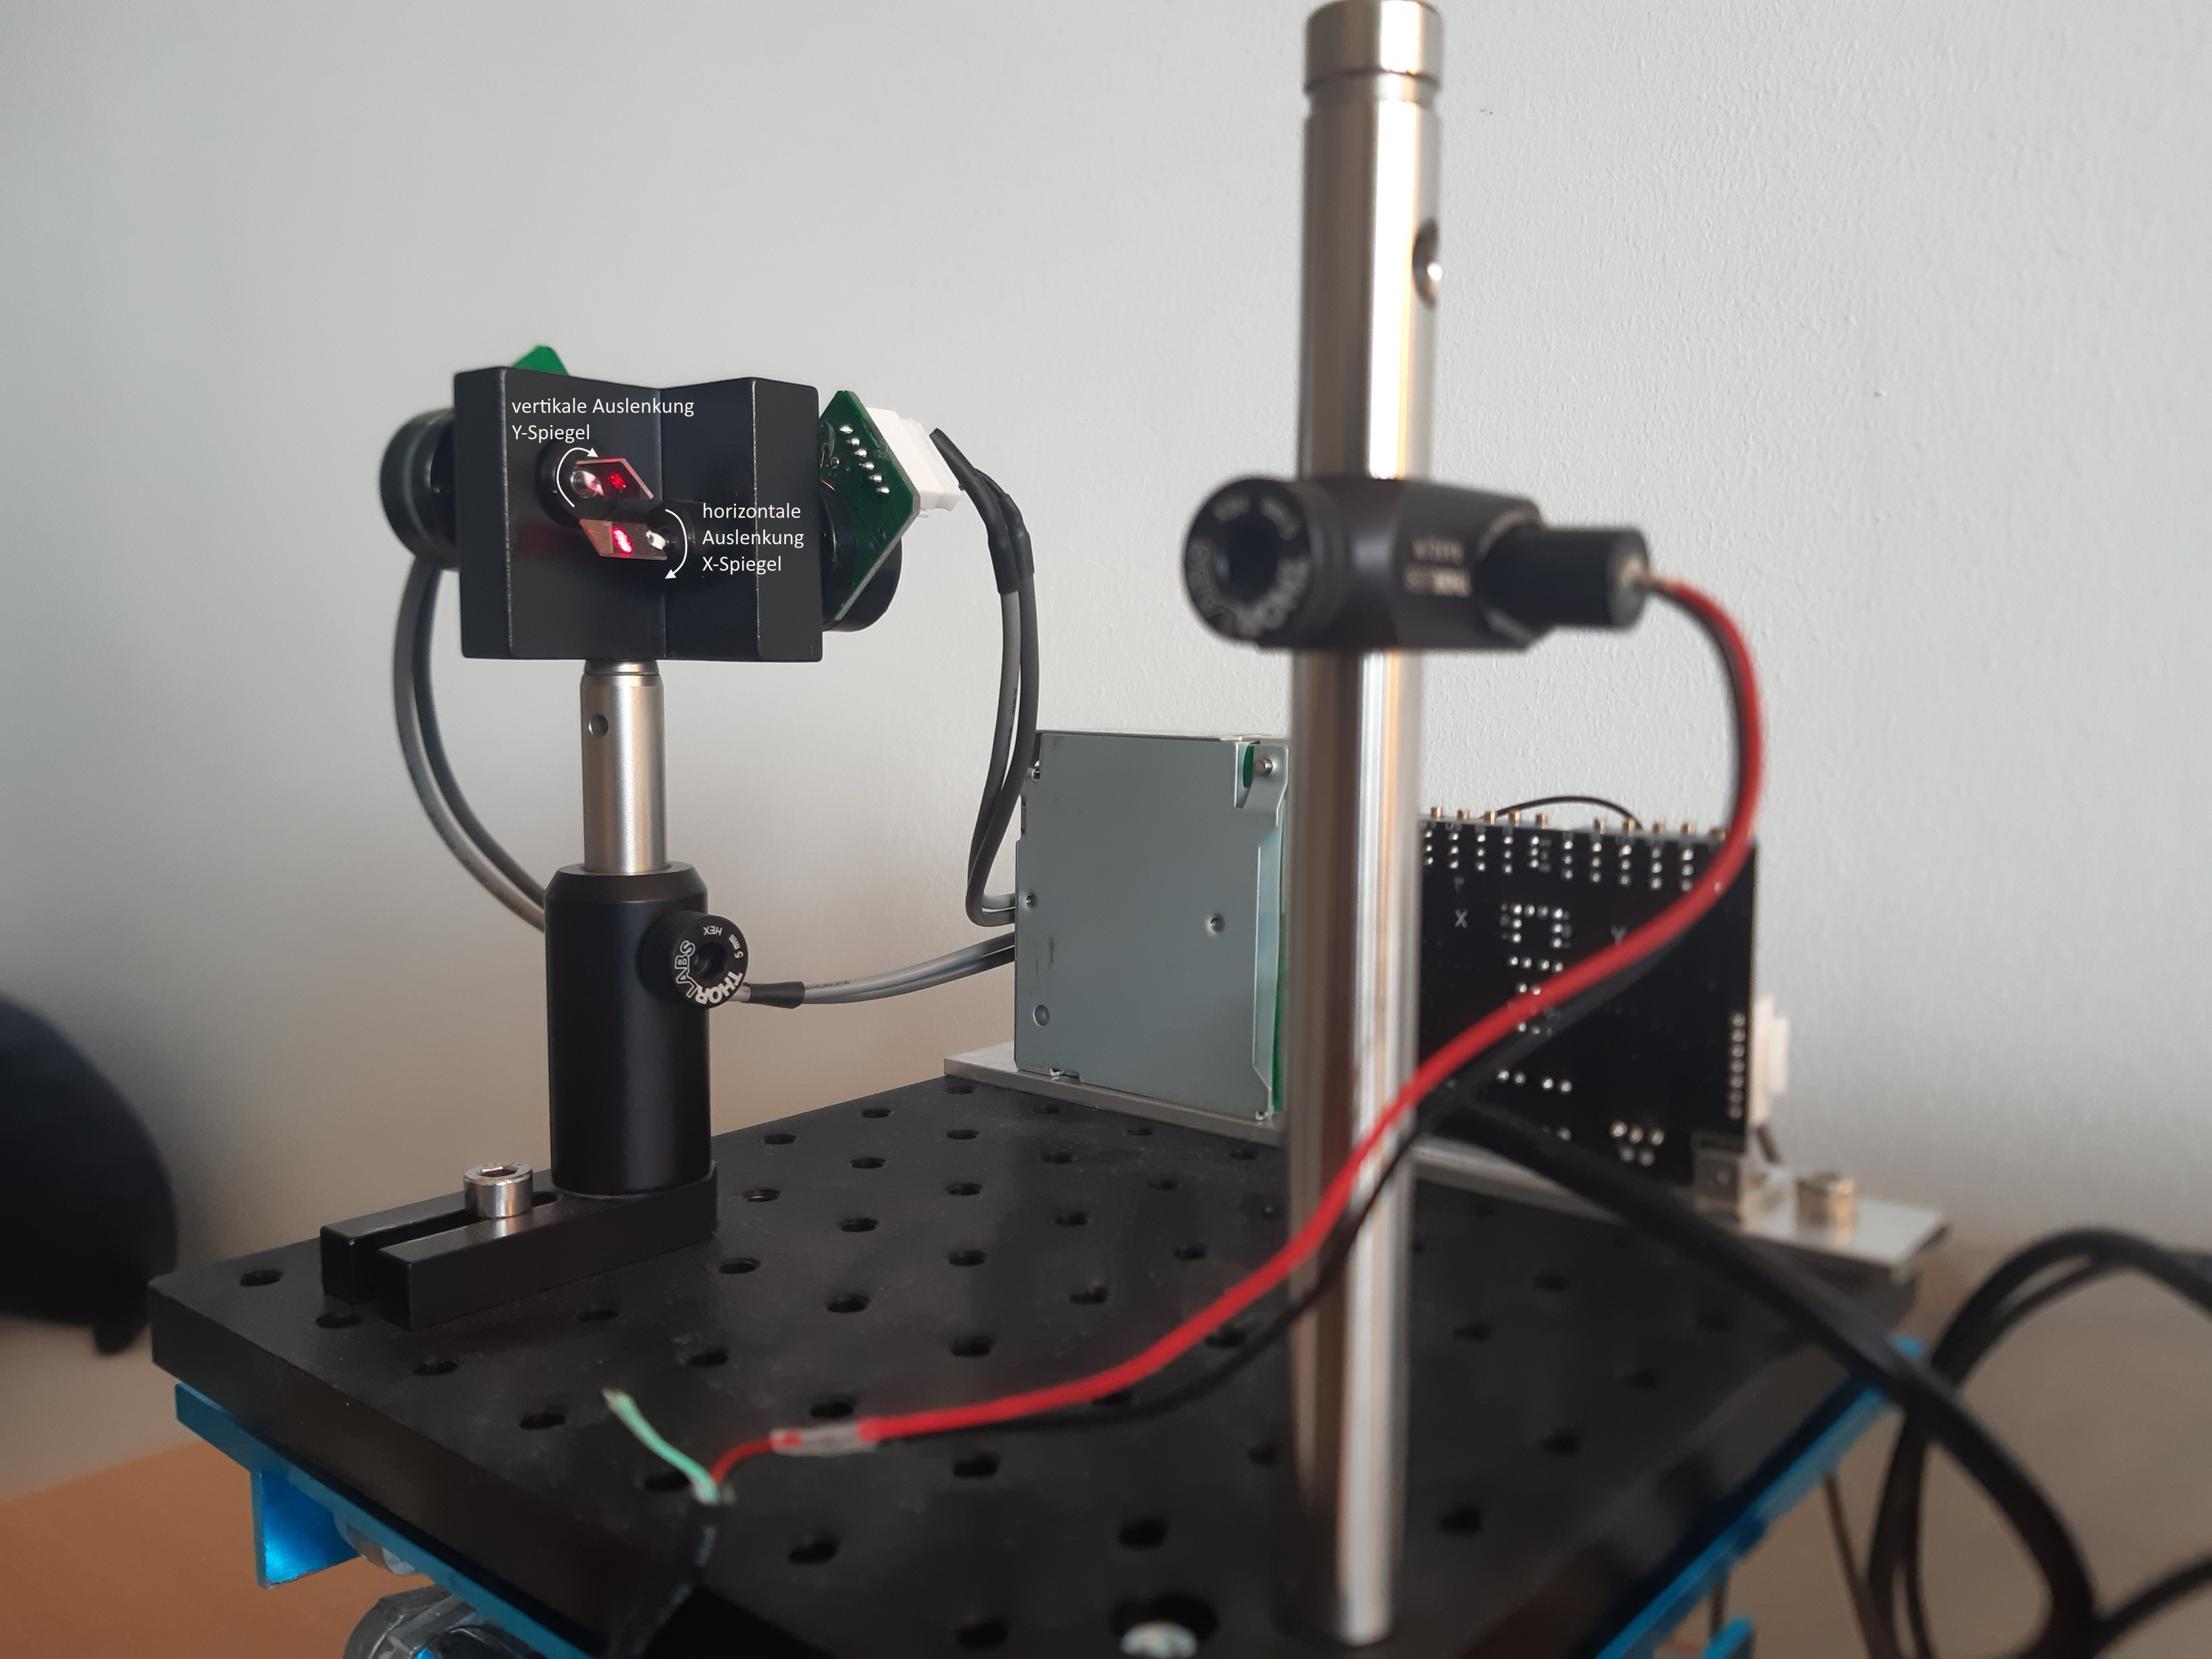
\includegraphics[width=\textwidth]{images/DetailGalvoOn.jpg}	\caption{DetailGalvoOn}	\label{DetailGalvoOn}	\end{figure}
\begin{figure}[h!]	\centering	\includegraphics[width=\textwidth]{images/DutTop02.jpg}	\caption{DutTop02}	\label{DutTop02}	\end{figure}

\section{Control of Galvanometer-Scanners}
Commercially available galvanometer scanners usually allow control in the form of analogue voltage inputs with a range of $\pm$ 10volts. The angle of the rotated mirror follows that control-voltage in a linear manner for sufficiently low frequencies. The signal-forms to result in the rectangular scan-grids, as described in the previous section, are depicted in fig.~\ref{GalvoRamps01}. To achieve these signals, a microcontroller-board was designed, including 16-bit analogue outputs, USB-connectivity and coaxial trigger outputs, among other features. To utilise these features and form an arbitrary signal generator for mentioned ramp-signals, a firmware is necessary. This should be done in a fashion employing quality-assurance during the implementation-process, as well as the verification-phase of the firmware and its supporting hardware. Aside from signal-generation and USB-connectivity, additional features are desirable, such as user-controllable relays, utilisation of watchdog-timer, UART-, I2C- and SPI-ports as well as analogue inputs. The combination of hard- and firmware will be called OCTane. Fig. ~\ref{blocktane} demonstrates the involvement of an OCTane into an OCT-system.
\bildGr{h!}{blocktane.pdf}{Integration of an OCTane}{blocktane}{0.75\textwidth}

\begin{figure}[h!]	\centering	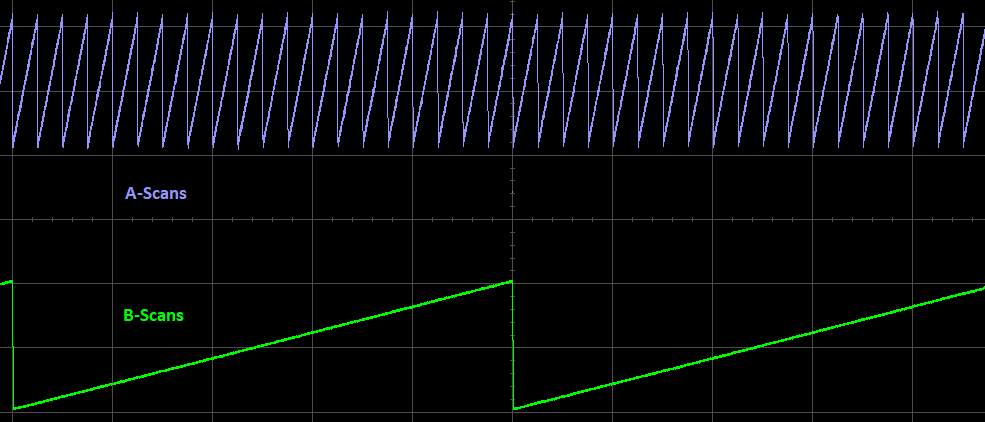
\includegraphics[width=\textwidth]{images/GalvoRamps01.png}	\caption{GalvoRamps01}	\label{GalvoRamps01}	\end{figure}
This leads to the scientific problem at hand: 
\begin{center} {\bf How can measures of quality be applied to a bare-metal firmware?}
\end{center}
% \subsection{optional: adapted steering curves}
% ...fliegt wohl raus
% \TODO{Modell ausm Paper per flachheitsbasierter Reglung auf Steuer-rampen draufrechnen}
% \textcolor{grey}{  }

% thethesis.tex
\chapter{Fundamentals}
\label{cha:Fundamentals}
	% Fundamentals
	\section{Code Quality}
	\subsection{Motivation}
As computers and microcontrollers are introduced into ever increasing application areas, the correct and reliable function of the software runing them becomes more important. A significantly increasing proportion of the development costs falling towards software, compared to hardware, suggests, to consider also the financial efforts put into testing and verification of said software. As the lifespan of software is significantly longer than the corresponding hardware, this seems to be a sensible investment. Nonetheless, reducing the costs for software development is also particularly economical. Investigating the dynamics of development costs leads to the result, that, the later in a project lifecycle, the higher the expenses. This means, that the largest portion of money is spent in the last phase, the maintenance of software, that is already in the market! This is a direct consequence of low quality standards applied to the product. More detailed expressed, errors are induced in the implementation, persist unnoticed through testing and verification. Finally, this erros appear as faults in operation at the customer site. Furthermore, if the project suffers from lazy documentation, insufficient structure, identifying these errors and correctiong them becomes consuming in time, cost and resources. This phenomenom is further escalated with the increasing complexity of todays software. An even worse phenomenon can arise: Insufficient understanding of a faulty piece of software at hand, can lead to introducing even more errors with additional code, that is actually intended to fix a bug. Especially when poor structuring masks hidden dependencies between modules. A general rule oh thumb here is: The earlier an error arises, for example in the phase of gathering requirements, the more extensive changes are necessary. In other words: The earlier an errors is induced and the later it is discovered, the more expensive are its consequences. 

But these problems have suitable solutions at hand. It is not compulsive to plunge money, hours and employee motivation on unnecessary maintenance. Employing the right methods, implemented software can become reliable, easy to change, inexpensive to maintain and allow a more intuitive understanding. Distinguischable into two categories, these methods are either analytical or constructive. Widespread examples are functional decomposition, object-oriented development, structured design, structured analysis or the use of the unified modeling language (\TODO{UML}).

% \textcolor{gray}{  functionally decomposing and object-oriented software development methods are particularly widespread. Examples are Structured Analysis (SA) /DeMarco 85/, Structured Design (SD) and the Unified Modeling Language (UML) /Booch et al. 98/. A comprehensive description of the development methods for software is contained in /Balzert 00/.}
Best practice is to employ a combination of constructive and analytical methods. Constructive means alone can assist in preventing errors in the intended product, but not guarantee their absence. Analytical means are capable of demonstrating the absence of errors, but not their prevention, so a large amount of preventable errors might emerge, when only analytical means are put to use. The combined use advisable would be, to employ constructive methods during every phase of a development project, and assessing the intermediate products with analytical methods by the end of each phase. This process is called the 'principle of integrated quality assurance' (cite: Liggesmeyer). If the predefined criteria for sufficient quality are not met by intermediate results, they are not transferred to the next phase and the recent phase has to further developed, until all hard criteria are met. This concept assists the development team in the early detection of errors and their removal at reasonable effort. Ideally all errors induced in a development phase are detected and eliminated by the end of the same phase. This should further help in minimizing the number of errors in a product over several phases.
The described process makes it evident, that testing only a finished product is no sufficient means of ensuring high quality. Already the first intermediate result has to be investigated for deviations from the quality goals and measures have to taken for correction at an early stage. Also an interaction between constructive and analytical quality measures is required. While constructive methods are advised during the implementation activities of a phase, it should be followed by the corresponding analysis.
% \textcolor{gray}{The interlocking of design and test steps is also possible in development processes that do not provide for any explicit phases (e.g. extreme programming). }
A key factor in ensuring the intended quality lies in the early definition of these quality goals. It constitutes not of defining the requirements, but the specification of the desired quality features. This has to happen even before the phase of requirement-definition, as the requirements themself are affecte by aformentioned quality goals. On the other hand, testing results against quality features is also of central importance. The typical approach of every devloper is, to call a written program with a few sets of inputs and observe the program for expected, or divergent behaviour. This already constitutes for an informal danymic test. Inspecting the code after, implementing it, for structural errors is the informal equivalent of a static analysis. As these informal methods are widespread among programmers, employing formal processes of testing is rather disregarded among programmers, as well as the knowledge about their effectiveness. Ideally, testing is aimed at generating reproducible results, while following well defined procedures.

In the course of this chapter, techniques, tools, and procedures are discussed, to ensure software quality from an analytical point of view. Testing techniques are the main focus here. Additionally to the class od danymic tests, static analysis as well as formal methods are discussed. While object-oriented techniques for design, programming and analysis are state-of-the-art among server- and desktop-applications, embedded projects still are not generally written, employing OOP-methods. Nevertheless, either object-oriented and ebedded aspects are discussed with regards to testing and quality assurance. Further aspects of embedded projets often are certain levels of security and reliability to be guaranteed by the software. So these apsects are discussed in an upcoming \TODO{chapter/subsection}.

Depending on the type of examination, supportive software-tools are necessary and will therfore be discussed. Certain techniques, like inspection and reviews are dedicated to be done wiht support ing tools, apart from editors for reading the code. Nontheless, both kinds of examination require organizational measures to be carried, defining responsibilities and procedures. The correct execution of these measures constitute the organizational framework of testing.

While hardware quality assurance often results in quantitative results, same is not the case for software, atl east not to the same extent as for hardware. But processes exist for both worlds, to ensure systematic development, as well as quality assurance. Developers of systems integrating both hardware and software have to be aware of their differences. Also, strictly separating the quality measures for software and hardware is not an advisible way to go. The quality properties have to be specified and verified for the complete system and not just its separate modules. The test results of individual modules, usually, can not be superimposed, but the correct behaviour of the whole system has to be demonstrated. \BLUE{Therefore, the deviating aspects of hardware and software quality assurance have to be examined.}
	
	\subsection{Terminology and definitions of terms}
	\subsubsection{Quality, Quality requirements, Quality features, Quality measures}
		\begin{itemize}
		\item {\bf Quality}, according to DIN 55350, is defined as: The ability of a unit, or device, to fulfill defined and derived quality requirements.
		\item {\bf Quality requirements} describes the aggregate of all single requirements regarding a unit or device.
		\item {\bf Quality features} describe concrete properties of a unit or device, relevant for the definition and assessment of the quality. While it does not make quantitative statements, or allowed values of a property, so to say, it very well may have a hierarchical structure: One quality feature, being composed of several detailed sub-features. A differentiation into functional and non-functional features is advised. Also features may have different importance for the customer and the manufacturer. Overarching all these aspects, features may interfere with eachother in an opposing manner. As a consequence, maximizing the overall level of quality, regarding every aspect, is not a feasable goal. The sensible goal is to find a trade-off between interfering features, and achieve a sufficient level of quality for all relevant aspects. Typical features, regarding software developmant include: Safety, security, reliability, dependability, availability, robustness, efficiency regarding memory and runtime, adaptability portability, and testability.
		\item {\bf Quality measures} define the quantitative aspects of a quality feature. These are measures, that allow conclusions to be drawn about the characteristics of certain quality features. For example, the MTTF (mean time to failure), is a widespread measure for reliability.
		\end{itemize}
	
	\bildGr{b!}{../images/ErrorFaultFailure.pdf}{Causal chain}{ErrorFaultFailure}{0.5\textwidth}

	\subsubsection{Error, Failure, Fault}
	\begin{minipage}{\linewidth}
	\begin{itemize}
		\item {\bf Error}, the root cause of a device or unit to fail, may originate from operation outside the specification, or from human mistakes in the design.
		\item {\bf Failure}, or defect is the incorrect internal state of a unit, and is the result of an error. It exists either on the hard- or software-side and is the cause of a fault, but not necessarily.
		\item {\bf Fault} is the incorrect behaviour of the unit, or it's complete cease of service, observable by the user. It is caused by a failure.
		\item These definitions are in accordance with \TODO{cite:[Kopetz/Millinger]} and have causal dependencies, depicted in Fig.~\ref{ErrorFaultFailure}.
		\item While an error can be classified by its persistence, being permanent or transient; Failures and Faults are classified more detailed into consistent/inconsistent, permanent/transient and benign/malign, among other categories.
	\end{itemize}
	\end{minipage}
	
	\subsubsection{Correctness}
		{\bf Correctness} is the binary feature of a unit or device, loosely described as 'the absence of failures'. A more specific description would be, that a correct software operates consistent to its specification. This implies, that no conclusion about correctness is possible, whithout an existing specification.
	\subsubsection{Completeness}
		{\bf Completeness} describes, that all functionalities, given in the specification are implemented. This includes normal intended operation, as well as the handling of error-states. It is a neccessary, but not a sufficient criterion for correctness.
	\subsubsection{Testability}
	{\bf Testability} describes the property of a unit, to include functionality dedicated only to facilitate the verification of said unit. Supporting concepts include the \\
	% \begin{minipage}{\linewidth}
	\begin{itemize}
		\item Partitioning of the whole unit into modules, that are testable in isolation. These modules should have little to no side-effects with eachother. 
		\item A dedicated debug-unit, making the actual state of the unit observable from outside further asists Testability. 
		\item Another concept is, to specify only as much input space as is necessary, resulting in fewer necessary test-cases to ensure a high coverage.
	\end{itemize}
	% \end{minipage}

	The aggregate of these concepts is called {\bf design-for-testability}.
	Generally, time-triggered units support testability to a higher degree, than event-triggered systems.
	\subsubsection{Safety and Security}
	% \begin{minipage}{\linewidth}
	\begin{itemize}
		\item {\bf Safety} means, that a unit is fit for its intended purpose and provides reliable operation within a specified load- and fault-hypothesis.
		\item {\bf Security}, though, is the resistance of unit against malicious and deliberate misusage.
	\end{itemize}
	% \end{minipage}
	\subsubsection{Reliability}
	{\bf Reliability} is a dynamic property, giving the probability, that a unit is operational after given time {\bf t}.
		\begin{align*}
		\textrm{Reliability ...} \quad R(t) & = e^{-\lambda (t-t_o) }\\
		\textrm{failure rate ...}  \quad \lambda & = \frac{1}{MTTF} 
		\end{align*}
	An exponential function, decaying from 100\% at time = t0, where a unit was known to be operating. $\lambda$ is the failure rate with dimension 'failures/h'
	
	\subsubsection{Maintainability}
	{\bf Maintainability} is the probabilty, that a system is repaired and functioning again within a given time after a failure. Note that this includes also the time required to detect the error.
	A quantified measure for it is the mean-time-to-repair (MTTR).
	\subsubsection{Availability}
	{\bf Availability} combines Reliability and Maintainability into a measure, giving the percentage of time, a unit is operational, providing full functionality.
		\begin{align*}
	\textrm{Availability ...} \quad A & = \frac{MTTF}{MTTF + MTTR}
		\end{align*}
	It is apparent, that a low time-to-repair and a high time-to-failure leads to high Availability.
	\subsubsection{\GREY{Robustness}}
	\subsubsection{Dependability}
	{\bf Dependability} finally, is composed of sufficiently fullfiled levels of \\
		% \begin{minipage}{\linewidth}
		\begin{itemize}
			\item Reliability
			\item Availability
			\item Maintainability
			\item Safety
		\end{itemize}
		% \end{minipage}
	...assembled into the common acronym {\bf R.A.M.S.}
	
	\subsubsection{load-hypothesis, fault-hypothesis}
	
	\subsection{Coverage metrics}
	
	\subsection{Reviews}
	
	\subsection{Load/Fault tests}
	
	\subsection{PM and ReqEng}
	
	\subsection{V-Model?}

	\section{Realtime and Reliability}
	\subsection{soft/firm/hard}
	\subsection{Jitter}
	\subsection{Timing}
	\subsubsection{Deadline}
	\subsubsection{Laxity}
	\subsubsection{Execution time}
	\subsection{Load/Fault Hypothesis}

	\section{Theory - CI/CD}
	\subsection{CI/CD with open source on BareMetal}
	\subsection{reliable USB-Connectivity}
	% \subsection{prepared for utilisation of complete Processor}
	% \section{Theory - Galvos}
	% \subsection{sensitive steering of Galvos}
	
	\chapter{Requirements}
	\label{cha:Requirements}
		Allgemeine REQs an FW, RT (und evtl design-for-testability)

	\chapter{Implementation}
	\label{cha:Implementation}
		\subsection{Concept}
		\subsubsection{FSM}
		\subsubsection{Trigger-Diagramme}

		\section{Hardware}
			\subsection{STM32F4}
			\subsection{Wandler, Level-Shifter, HighSider}

		\section{Software tools}
			\subsection{CubeIDE}
			\subsection{gcov}
			\subsection{valgrind}
			\subsection{gitlab}
			\subsection{runner}
			\subsection{HIL-Setup}
			
		\section{Firmware-Requirements}
			\subsection{FW-REQ}
			\subsection{load-hypothesis, fault-hypothesis}
			\subsection{Traceability-Matrix}
			Linking Requirements by there tags, to the SW-modules, where they are fulfilled
			\subsection{TCs}
			\subsection{Unit-Tests}
			\subsection{Module-Tests}
			\subsection{Integration-Tests}
			\subsection{Load/Fault Tests}
			
		
	\chapter{Results}
	\label{cha:Results}
		% Results
		\section{Test-Res}
		\section{Coverages}
		\section{Review-remakrs}
		\section{Gavlo-Performance}
	% thethesis.tex


\chapter{Fundamentals}
\label{cha:Fundamentals}
	% Fundamentals
	\section{Code Quality}
	\subsection{Motivation}
As computers and microcontrollers are introduced into ever increasing application areas, the correct and reliable function of the software runing them becomes more important. A significantly increasing proportion of the development costs falling towards software, compared to hardware, suggests, to consider also the financial efforts put into testing and verification of said software. As the lifespan of software is significantly longer than the corresponding hardware, this seems to be a sensible investment. Nonetheless, reducing the costs for software development is also particularly economical. Investigating the dynamics of development costs leads to the result, that, the later in a project lifecycle, the higher the expenses. This means, that the largest portion of money is spent in the last phase, the maintenance of software, that is already in the market! This is a direct consequence of low quality standards applied to the product. More detailed expressed, errors are induced in the implementation, persist unnoticed through testing and verification. Finally, this erros appear as faults in operation at the customer site. Furthermore, if the project suffers from lazy documentation, insufficient structure, identifying these errors and correctiong them becomes consuming in time, cost and resources. This phenomenom is further escalated with the increasing complexity of todays software. An even worse phenomenon can arise: Insufficient understanding of a faulty piece of software at hand, can lead to introducing even more errors with additional code, that is actually intended to fix a bug. Especially when poor structuring masks hidden dependencies between modules. A general rule oh thumb here is: The earlier an error arises, for example in the phase of gathering requirements, the more extensive changes are necessary. In other words: The earlier an errors is induced and the later it is discovered, the more expensive are its consequences. 

But these problems have suitable solutions at hand. It is not compulsive to plunge money, hours and employee motivation on unnecessary maintenance. Employing the right methods, implemented software can become reliable, easy to change, inexpensive to maintain and allow a more intuitive understanding. Distinguischable into two categories, these methods are either analytical or constructive. Widespread examples are functional decomposition, object-oriented development, structured design, structured analysis or the use of the unified modeling language (UML).

\textcolor{gray}{  functionally decomposing and object-oriented software development methods are particularly widespread. Examples are Structured Analysis (SA) /DeMarco 85/, Structured Design (SD) and the Unified Modeling Language (UML) /Booch et al. 98/. A comprehensive description of the development methods for software is contained in /Balzert 00/.}
Best practice is to employ a combination of constructive and analytical methods. Constructive means alone can assist in preventing errors in the intended product, but not guarantee their absence. Analytical means are capable of demonstrating the absence of errors, but not their prevention, so a large amount of preventable errors might emerge, when only analytical means are put to use. The combined use advisable would be, to employ constructive methods during every phase of a development project, and assessing the intermediate products with analytical methods by the end of each phase. This process is called the 'principle of integrated quality assurance' (cite: Liggesmeyer). If the predefined criteria for sufficient quality are not met by intermediate results, they are not transferred to the next phase and the recent phase has to further developed, until all hard criteria are met. This concept assists the development team in the early detection of errors and their removal at reasonable effort. Ideally all errors induced in a development phase are detected and eliminated by the end of the same phase. This should further help in minimizing the number of errors in a product over several phases.
The described process makes it evident, that testing only a finished product is no sufficient means of ensuring high quality. Already the first intermediate result has to be investigated for deviations from the quality goals and measures have to taken for correction at an early stage. Also an interaction between constructive and analytical quality measures is required. While constructive methods are advised during the implementation activities of a phase, it should be followed by the corresponding analysis.
\textcolor{gray}{The interlocking of design and test steps is also possible in development processes that do not provide for any explicit phases (e.g. extreme programming). }
A key factor in ensuring the intended quality lies in the early definition of these quality goals. It constitutes not of defining the requirements, but the specification of the desired quality features. This has to happen even before the phase of requirement-definition, as the requirements themself are affecte by aformentioned quality goals. On the other hand, testing results against quality features is also of central importance. The typical approach of every devloper is, to call a written program with a few sets of inputs and observe the program for expected, or divergent behaviour. This already constitutes for an informal danymic test. Inspecting the code after, implementing it, for structural errors is the informal equivalent of a static analysis. As these informal methods are widespread among programmers, employing formal processes of testing is rather disregarded among programmers, as well as the knowledge about their effectiveness. Ideally, testing is aimed at generating reproducible results, while following well defined procedures.

In the course of this chapter, techniques, tools, and procedures are discussed, to ensure software quality from an analytical point of view. Testing techniques are the main focus here. Additionally to the class od danymic tests, static analysis as well as formal methods are discussed. While object-oriented techniques for design, programming and analysis are state-of-the-art among server- and desktop-applications, embedded projects still are not generally written, employing OOP-methods. Nevertheless, either object-oriented and ebedded aspects are discussed with regards to testing and quality assurance. Further aspects of embedded projets often are certain levels of security and reliability to be guaranteed by the software. So these apsects are discussed in an upcoming \TODO{chapter/subsection}.

Depending on the type of examination, supportive software-tools are necessary and will therfore be discussed. Certain techniques, like inspection and reviews are dedicated to be done wiht support ing tools, apart from editors for reading the code. Nontheless, both kinds of examination require organizational measures to be carried, defining responsibilities and procedures. The correct execution of these measures constitute the organizational framework of testing.

While hardware quality assurance often results in quantitative results, same is not the case for software, atl east not to the same extent as for hardware. But processes exist for both worlds, to ensure systematic development, as well as quality assurance. Developers of systems integrating both hardware and software have to be aware of their differences. Also, strictly separating the quality measures for software and hardware is not an advisible way to go. The quality properties have to be specified and verified for the complete system and not just its separate modules. The test results of individual modules, usually, can not be superimposed, but the correct behaviour of the whole system has to be demonstrated. \BLUE{Therefore, the deviating aspects of hardware and software quality assurance have to be examined.}
	
	\subsection{Terminology and definitions of terms}
	\subsubsection{Quality, quality requirement, quality feature, quality measure}
		\begin{itemize}
		\item For the term 'quality', the definition according to DIN 55350 is used: The ability of a unit, or device, to fulfill defined and derived quality requirements.
		\item Quality requirements again, describes the aggregate of all single requirements regarding a unit or device.
		\item A quality feature describes concrete properties of a unit or device, relevant for the definition and assessment of the quality. While it does not make quantitative statements, or allowed values of a property, so to say, it very well may have a hierarchical structure: One quality feature, being composed of several detailed sub-features. A differentiation into functional and non-functional features is advised. Also features may have different importance for the customer and the manufacturer. Overarching all these aspects, features may interfere with eachother in an opposing manner. As a consequence, maximizing the overall level of quality, regarding every aspect, is not a feasable goal. The sensible goal is to find a trade-off between interfering features, and achieve a sufficient level of quality for all relevant aspects. Typical features, regarding software developmant include: Safety, security, reliability, dependability, availability, robustness, efficiency regarding memory and runtime, adaptability portability, and testability.
		\item Finally, the quality measure defines the quantitative aspects of a quality feature. These are measures, that allow conclusions to be drawn about the characteristics of certain quality feature. Foe example, the \TODO{ ~ref{} } MTTF (mean time to failure), is a widespread measure for reliability.
		\end{itemize}

	\subsubsection{error, failure, fault}
	\begin{itemize}
		\item Error, the root cause of a device or unit to fail, may originate from human mistakes or from its operation outside the specification.
		\item Failure, or defect is the incorrect state of a unit, either on the hard- or software-side. It may cause a fault, but not necessarily.
		\item Fault is the incorrect behaviour of the unit, or it's complete cease of service, observalbe by the user.
		\item \TODO{Die drei Begriffe aufpaepeln mit deifitione  laut Leveson/Millinger}
		\item Whereas these three terms have differnt definitions in varying publications, the afformentioned declarations seem to be best suited for devices containing substantiable amount of software.
		\end{itemize}
	
	\subsubsection{correctness}
		Correctness is the binary feature of a unit or device, loosely described as 'the absence of failures'. \TODO{da is noch mher beim Liggesmayer}
	\subsubsection{completeness}
		Completeness describes, that all functionalities, given in teh specification are implemented. This includes normal intended operation, as well as the handling of error-states.
	\subsubsection{security}
	\subsubsection{Reliability}
	\subsubsection{Availability}
	\subsubsection{Robustness}


	\subsection{Coverage metrics}
	
	\subsection{Reviews}
	
	\subsection{Load/Fault tests}
	
	\subsection{PM and ReqEng}
	
	\subsection{V-Model?}

	\section{Realtime and Reliability}
	\subsection{soft/firm/hard}
	\subsection{Jitter}
	\subsection{Zeitpunkte}
	\subsubsection{deadline}
	\subsubsection{laxity}
	\subsubsection{execution time}
	\subsection{Load/Fault Hypothesis}

	\section{Theory - CI/CD}
	\subsection{CI/CD with open source on BareMetal}
	\subsection{reliable USB-Connectivity}
	% \subsection{prepared for utilisation of complete Processor}
	% \section{Theory - Galvos}
	% \subsection{sensitive steering of Galvos}
	
\chapter{Requirements}
\label{cha:Requirements}
	Allgemeine REQs an FW, RT (und evtl design-for-testability)

\chapter{Implementation}
\label{cha:Implementation}
	\subsection{Concept}
	\subsubsection{FSM}
	\subsubsection{Trigger-Diagramme}

	\section{Hardware}
		\subsection{STM32F4}
		\subsection{Wandler, Level-Shifter, HighSider}

	\section{Software tools}
		\subsection{CubeIDE}
		\subsection{gcov}
		\subsection{valgrind}
		\subsection{gitlab}
		\subsection{runner}
		\subsection{HIL-Setup}
		
	\section{Firmware-Requirements}
		\subsection{FW-REQ}
		\subsection{Traceability-Matrix}
		Linking Requirements by there tags, to the SW-modules, where they are fulfilled
		\subsection{TCs}
		\subsection{Unit-Tests}
		\subsection{Module-Tests}
		\subsection{Integration-Tests}
		\subsection{Load/Fault Tests}
		
	
\chapter{Results}
\label{cha:Results}
	% Results
	\section{Test-Res}
	\section{Coverages}
	\section{Review-remakrs}
	\section{Gavlo-Performance}
	


% \chapter{Figures, Tables, Source Code}
\label{cha:Figures}

% \chapter[Mathematical Elements]{Mathematical Elements, Equations and Algorithms}
\label{cha:Mathematics}


% \chapter[Using Literature]{Using Literature and other Resources}
\label{cha:Literature}

The APA citation style%
\footnote{\url{https://apastyle.apa.org/style-grammar-guidelines/references/}}
requires different citation macros, depending on the usage and the
occurrence of the reference in the text.

\section{Narrative Citations}

In narrative references, the source is used as the subject or object of the sentence. The
year is placed after the author's name in parentheses. To create this kind of citation use 
%
\begin{itemize}
\item[] \verb!\textcite{!\textit{keys}\verb!}!.
\end{itemize}
%
\textbf{Example:}
\textcite{Daniel2018} give a brief introduction to \latex, whereas \textcite{Oetiker2021, Kopka2003} 
go into more detail.


\section{Narrative Citations within Parentheses}

If a reference is to be used within parentheses, these must be omitted from the reference itself. 
The associated macro is
%
\begin{itemize}
\item[] \verb!\nptextcite{!\textit{keys}\verb!}!.
\end{itemize}
%
\textbf{Example:}
In any case, it is recommended to obtain literature on the topic of \latex (\eg, 
\nptextcite{Daniel2018, Oetiker2021, Kopka2003}).


\section{Parenthetical Citations}

Parenthetical citations are used when the reference should be cited at the end of a sentence or statement.
The author's name and year are enclosed in parentheses and separated by a comma. In this case use
%
\begin{itemize}
\item[] \verb!\parencite{!\textit{keys}\verb!}!.
\end{itemize}
%
\textbf{Example:}
For \latex, there are short introductions \parencite{Daniel2018}, as well as more comprehensive works 
\parencite{Oetiker2021, Kopka2003}.




% \chapter{galvoChar}
\newcommand \galvo {Galvanometer-Spiegel}
\newcommand \bildwidth {0.95\textwidth}

% bild{h!}{}{}{}
% #1 float position
% #2 filename.ext
% #3 cap
% #4 label
\newcommand \bild[4]{\begin{figure}[#1]	\centering	\includegraphics[width=\bildwidth]{pics/#2}	\caption{#3}	\label{#4}	\end{figure}}


% \begin{abstract}
OCT-Systeme (optical coherence tomography) ermitteln punktweise, tiefenaufgeloeste Geometrie-Daten in transparenten Materialien. Zur Ermittlung von 3-dimensionalen Datensaetzen wird der Messpunkt dabei mit \galvo n im X/Y-Betrieb verfahren. Dies sind hochdynamische Drehantriebe fuer optische Anwendungen, die mit einer Rate von etwa 500Hz vor- und rueckwaerts rotieren koennen. Sie tragen mitrotierende Spiegel, um den optischen Pfad auszulenken und somit flaechige Scans zu ermoeglichen. \\ 
Handelsuebliche Galvanometer-Spiegel besitzen mechanische Traegheiten, die bei Scan-Raten ab 800Hz keine maximale Auslenkung mehr erlauben. Dadurch wird bei hohen Geschwindigkeiten der optische Messbereich eingeschraenkt. An realen, vorhandenen \galvo wird durch Messungen diese Traegheit charakterisiert und modelliert. Dieses Modell soll als Basis dienen, um adaptierte Steuersignale zu erzeugen, die die angesprochenen Traegheiten Ausgleichen.\\
% \end{abstract}

% \begin{IEEEkeywords}
OCT-System, Galvanometer-Scanner, Regelungstechnik, Laser-Scanner, Interferometrie, dynamische Modellierung
% \end{IEEEkeywords}

% \section{Einleitung}
	% \subsection{Optische Kohaerenz-Tomographie}
% Optische Kohaerenz Tomographie (optical coherence tomography, OCT) ist ein bildgebendes Messverfahren zur Analyse von transparenten und opaken Materialien und weist aehnlichkeiten zu den Messprozessen via Ultraschall oder Radar auf. Die Probe, die vermessen werden soll, wird mit einer elektromagnetischen Welle beaufschlagt, die resultierenden 'Echos' werden bezueglich ihrer resultierenden Laufzeiten analysiert. Aus diesen Laufzeiten wiederum ergibt sich die geometrische Struktur, die den Schichtaufbau der Probe, oder auch die maximale Eindringtiefe der Welle enthaelt. So entsteht ein tiefenaufgeloester Messpunkt. In der Regel wird diese EM-Welle aus einer kohaerenten, breitbandigen Lichtquelle im sichtbaren bis in den nahen Infrarot-Bereich erzeugt. Kohaerenz bedeutet, dass mehrere Wellenzuege einer Lichtquelle eine feste Phasenbeziehung zueinander haben muessen. Dies ist notwendig, um stabile Interferenzmuster zu erhalten. Zur Detektion der Echos reichen jedoch keine herkoemmlichen Opto-Detektoren oder Kameras aus, einerseits aufgrund der Ausbreitungsgeschwindigkeit des Lichtes, andererseits an den geringen reflektierten Lichtintensitaeten. Deshalb kommt Interferometrie zum Einsatz, um die Eindringtiefe eines Photons zu ermitteln, das von einer Probe reflektiert wird. \\ Bei Interferometrie wird der Laserstrahl gesplittet und eine Welle auf einen optischen Referenzenpfad bekannter Laenge gesendet, die andere auf die Oberflaeche des Prueflings. Die Reflexionen, also die ruecklaufenden Wellen werden ueberlagert und erzeugen je nach Beschaffenheit des Probenmaterials konstruktive oder destruktive Interferenz. Diese Interferenz kann mittels eines Opto-Detektors\footnote{time-domain OCT, swept-source},  oder eines Spektrometers\footnote{ spectral domain - OCT }  gesampelt und weiterverarbeitet werden. Ein einzelner vermessener Punkt und seine Tiefeninformation ueber das betrachtete Material wird als A-Scan bezeichnet. Aggregiert man eine Menge von A-Scans entlang einer Linie (X-Richtung) ueber das Probenmaterial, bildet dies einen B-Scan und die Aggregation von B-Scans entlang einer Linie in Y-Richtung ergibt einen Volumen-Scan, also ein raeumliches, ein dreidimensionales Abbild des Probenmaterials. Relevante Parameter von OCT-Systemen sind die Eindringtiefe, der axiale und laterale Messbereich, axiale und laterale Aufloesung und die Messgeschwindigkeit. Betraegt die Eindringtiefe bei Ultraschall typischerweise einige Zentimeter und eine Aufloesung im Millimeter-Bereich, so erlaubt OCT nur wenige Millimeter unter die Oberflaeche zu schauen, jedoch mit Mikrometer-Aufloesungen. Abmessbare Bereiche bewegen sich bei Ultraschall in der Groessenordnung von Zentimetern, bei OCT in Millimetern\cite{WhitepaperEO}. Erreichbare Geschwindigkeiten ergeben sich aus A-Scan-Raten bis 100kHz. \\  
Die Bezeichnung 'optische Kohaerenz-Tomographie' ergibt sich einerseits aus der kohaerenten Lichtquelle. Andererseits stehen die Namensteile 'tomos' fuer Schnitt oder Sektion, und 'graphein' fuer Schreiben oder Zeichnen, und stammen beide aus dem Griechischen. Sie spiegeln wider, dass das entstehende Abbild aus einzelnen Sektionen oder Schnittbildern zusammengesetzt wird. Das Manipulieren des Lichtstrahls entlang der erwaehnten Linien erfolgt mit rotierbar gelagerten Spiegeln, einen fuer die X- einen fuer die Y-Richtung. Je schneller diese Rotation moeglich ist, desto schneller koennen OCT-Bilder erstellt werden. Eine weitverbreitete technische Realisierung, die sehr schnelles Rotieren der Spiegel erlaubt, heisst \galvo .
\bild{h!}{DetailGalvoOn}{Anordnung von XY-\galvo n}{DetailGalvoOn}

% \subsection{ \galvo }
% Bei \galvo n (auch: Galvos) handelt es sich um hochdynamische opto-mechanische Komponenten, die auf dem klassischen Galvanometer nach Hans Christian Oersted basieren: Ein rotierbar gelagertes, magnetisierbares Objekt, zB. eine Magnetnadel, wird in der Naehe eines stromdurchflossenen Leiters aus seiner Ruhelage ausgelenkt. Die geringe Empfindlichkeit der Auslenkung gegenueber dem Strom wird verbessert, indem eine hohe Wicklungszahl des elektr. Leiters um das auszulenkende Objekt gelegt wird und somit eine elektrische Induktivitaet, eine Spule, entsteht. Der nichtlineare Zusammenhang zwischen Strom und Auslenkwinkel kann durch Lagerung der Spule zwischen einem starr angebrachten Eisenzylinder innerhalb und einem Dauermagneten, der ausserhalb der Spule angeordnet ist, in guter Naeherung linearisiert werden\cite{keithleyHistory}. Wird dieses klassische Galvanometer mit einem Spiegel als rotierbares Objekt erweitert, lassen sich damit optische Pfade, konkret: der Strahlengang einer punktfoermigen Lichtquelle in einer Raumdimension manipulieren. Praktikabel fuer technische Anwendungen ist, dass diese Manipulation einigermassen linear per Strom oder Spannung an der Galvo-Spule gesteuert werden kann. Bei den vorliegenden \galvo n ist eine Leistungselektronik enthalten, die fuer die Umsetzung von Steuersignalen auf die erforderlichen Stroeme und Spannungen sorgt, im Folgenden wird deshalb nurmehr von Steuersignalen gesprochen. Kombiniert man zwei \galvo n in geeigneter geometrischer Anordnung und bestrahlt diese mit einem Punktlaser, so laesst sich dieser Punkt im 2-Dimensionalen manipulieren. Eine solche Anordnung ist in Abb.~\ref{DetailGalvoOn} dargestellt. Bei ausreichender Geschwindigkeit, mit der der Laser-Punkt ausgelenkt wird, koennen 2D-Konturen projiziert werden, die fuer das menschliche Auge ein 'stehendes' Bild darstellen. So werden diese Komponenten fuer Laser-Shows eingesetzt. Handelsueblich werden diese Komponenten als Laser-Scanner bezeichnet und fuer Lichteffekte bei Musikveranstaltungen, Kunst-Installationen und Diskotheken eingesetzt. Auf OCT-Systeme appliziert, koennen Galvanometer-Spiegel hingegen genutzt werden, um die optische Wirkung einer kohaerenten Lichtquelle nicht auf einen Ortspunkt beschraenkt zu nutzen, sondern auf einer gewisse Flaeche verteilt an eine beliebige Stelle einer zu untersuchenden Probe zu projizieren. Werden ein X- und ein Y-Galvo jeweils mit einer langsamen und einer schnellen Rampe angesteuert, ergibt dies ein Rechteck auf der Probe, die gewuenschte 'Bildform' des Laserpunktes fuer OCT-Systeme. So koennen Proben rasterfoermig abgescannt werden.

\subsection{Motivation}
Die beschriebenen Eigenschaften, speziell der lineare Zusammenhang, gelten, bei guenstigen handelsueblichen \galvo n aus der Showlaser-Branche, fuer langsame Auslenkungen von $\le$800Hz. Schnellere Steuersignale fuehren zwar auch zu schnelleren Rotationen und erlauben somit schneller Messungen. Jedoch folgt die innere Mechanik des Spiegels dann  nicht mehr mit dem vollen Auslenk-Winkel. Auf eine technische Anwendung umgelegt, bedeutet dies, dass dann nicht mehr die volle Flaeche abgerastert werden kann. Offensichtlich liegt dies an der Massentraegheit der rotierbaren Komponenten, vermutet wird ein Tiefpass-Verhalten zwischen Steuersignal und Auslenkwinkel. Dieser Zusammenhang wird im Folgenden experimentell untersucht, um konkrete Aussagen ueber die Traegheit und deren Konsequenzen machen zu koennen und weiters, um mit adaptierten Steuersignalen auch bei hoeheren Frequenzen ($\sim 1000 ... 3500Hz$) volle Auslenkwinkel nutzen zu koennen. Abb.~\ref{SawVsSpline} zeigt ein moegliches adaptiertes Steuersignal. Das unterstellte Tiefpass-Verhalten wuerde auch eine Phasenverschiebung zwischen Steuersignal und Winkel implizieren, die ebenfalls untersucht wird.
\bild{h!}{SawVsSpline.eps}{bestehendes und adaptiertes Steuersignal}{SawVsSpline}
% \footnote{Diskotheken, Konzerte, Kunstinstallationen}
\section{Recherche}
\subsection{dynamisches Modell}
Die Modellierung erfolgt auf Basis experimenteller Untersuchung des Zusammenhangs zwischen Steuerspannung und Auslenkwinkel mit Methoden der Regelungstechnik. Einen vergleichbaren Ansatz haben Rasoanarivo et al. \cite{SLMGalvos:Rasoanarivo} gewaehlt, um Galvanometer-Spiegel zur Anwendung beim selektiven Laserschmelzen in der additiven Fertigung zu untersuchen. Dort wurde das bewegliche System als Gleichstrommotor mit uebertragungsfunktion 2ter-Ordnung modelliert. Selbigen Ansatz legt auch die Regelungstechnik nahe: Die beweglichen Komponenten werden als rotatorisches Starrkoerper-System angesehen, das ueber elektrische Induktion angeregt wird. Eine dynamische Vermessung per Sprungantwort eruebrigt sich, da zur Detektion notwendiges Equipment, zum Beispiel eine High-Speed-Kamera, nicht zur Verfuegung steht. Stattdessen fiel die Entscheidung auf Anregung mit Sinus-Signalen schrittweise steigender Frequenz und Aufnahme der resultierenden Projektion eines so abgelenkten Laserstrahles.
\subsubsection{	kpps versus dynamisches Modell}
In der Branche der Showlaser, aus der das Testobjekt stammt, ist zur Charakterisierung die Einheit 'kpps' gebraeuchlich und steht fuer 'kilo points per second', also wievielmal tausend Bildpunkte pro Sekunde projiziert werden koennen\cite{ildaHomepage}. Genaugenommen lautet die Bezeichnung 'kpps@8gradILDA' und bezieht sich auf eine Auslenkung von 8grad und Darstellung eines Testbildes nach ILDA\footnote{International Laser Display Association, definiert Standards fuer Showlaser}. Dies mag die Tauglichkeit eines \galvo s fuer Laser-Shows ausreichend beschreiben, ist jedoch fuer die Anwendung in OCT-Systemen nicht aussagekraeftig, da Dynamik in der Form 'Punkte pro Zeiteinheit' auf den gewuenschten kontinuierlichen Betrieb nicht umlegbar ist. Insbesondere, da in dieser Kennzahl Traegheiten sowohl fuer x- als auch y-Achse vermengt sind. Ausserdem wird auch nur der lineare Bereich getestet. Da dies die einzige dynamische Kennzahl von Schowlaser-\galvo n ist, bleibt nichts anders uebrig als selbst zu messen und zu modellieren.
% \subsection{ebay vs Sino vs Camebridge}
\section{Messungen}
Beim Testobjekt handelt es sich um einen 'RGB-SCAN20, 20Kpps galvanometer scanner', der Marke 'RGB-lasers'. Die Aufnahme der Auslenkungs-Amplitude erfolgt durch Vermessen des projizierten Laserpunktes mit Massband und freiem Auge, der Phasenlage durch einen Opto-Detektor, der auf der '0'-Linie des Strahlengangs sitzt. Abb.~\ref{ImageMeasure01} zeigt das ablesbare Amplituden-Bild einer Messung. Die kohaerenten Lichtquellen, die ueblicherweise in OCT-Systemen zum Einsatz kommen, sind nicht im menschlich sichtbaren Bereich verfuegbar, weshalb stattdessen ein roter Punkt-Laser zum Einsatz kommt. Auch saemtliche Komponenten der Interferometrie und deren Detektion tragen nichts zur Analyse der Galvo-Dynamik bei und sind deshalb nicht Teil der Messungen. Abb.~\ref{DutTop02} zeigt die Aufspannung des Testobjekts links, der Laser-Lichtquelle rechts, sowie der Treiber-Elektronik, ueber die Sinus-Signale auf das Testobjekt appliziert werden.
\begin{figure}[h!]	\centering	\includegraphics[width=\bildwidth]{pics/DutTop02.jpg}	\caption{Aufspannung des Testobjekts}	\label{DutTop02}	\end{figure}
\subsection{Konzept}
Um Messdaten fuer das Modell zu erhalten, werden die Galvanometer-Spiegel mit einem Laser-Strahl beleuchtet, wodurch diese in Ruheposition den Strahl rechtwinkelig umlenken und einen Laser-Punkt auf eine gegenueberliegende Flaeche projizieren. Weiters werden die Galvanometer-Spiegel separat mit sinusfoermigen Signalen angesteuert, wodurch ihre Spiegel rotiert werden. Dadurch wird der Punkt in x-, respektive, y-Richtung ausgelenkt. Bei langsamer Auslenkung mit einem Sinus von $\sim$1Hz bleibt die Projektion fuer das menschliche Auge noch deutlich als Punkt erkennbar, ab 5Hz entsteht der Eindruck einer ruckelnden Linie und bei 40Hz eine deutlich sichtbare Linie ohne erkennbares Zittern. Die Geometrie aus Messaufbau und Projektionsflaeche wird konstant gehalten und die Hoehe dieser Linie als Auslenkung herangezogen. Weiters wird im Punkt des Nulldurchgangs ein Opto-Detektor platziert, mit dem die Phasenlage des Laser-Strahl zum Steuersignal in Bezug gesetzt wird, dargestellt in Abb.~\ref{DetektorsForPhase}. Da das verwendete Massband eine spuerbare Flexibilitaet aufweist, wurde es auf Masshaltigkeit ueberprueft. Per Schieblehre nachgemessen, hat es nach dem Aufkleben auf eine Projektionsflaeche eine Abweichung $\le$ 1mm. Der Normalabstand zwischen Messobjekt und Projektionsflaeche betraegt 3200mm.
% \subsection{Aufbau}
	% \begin{equation}
	% d = 3190mm
	% \end{equation}
% \begin{figure}[h!]	\centering	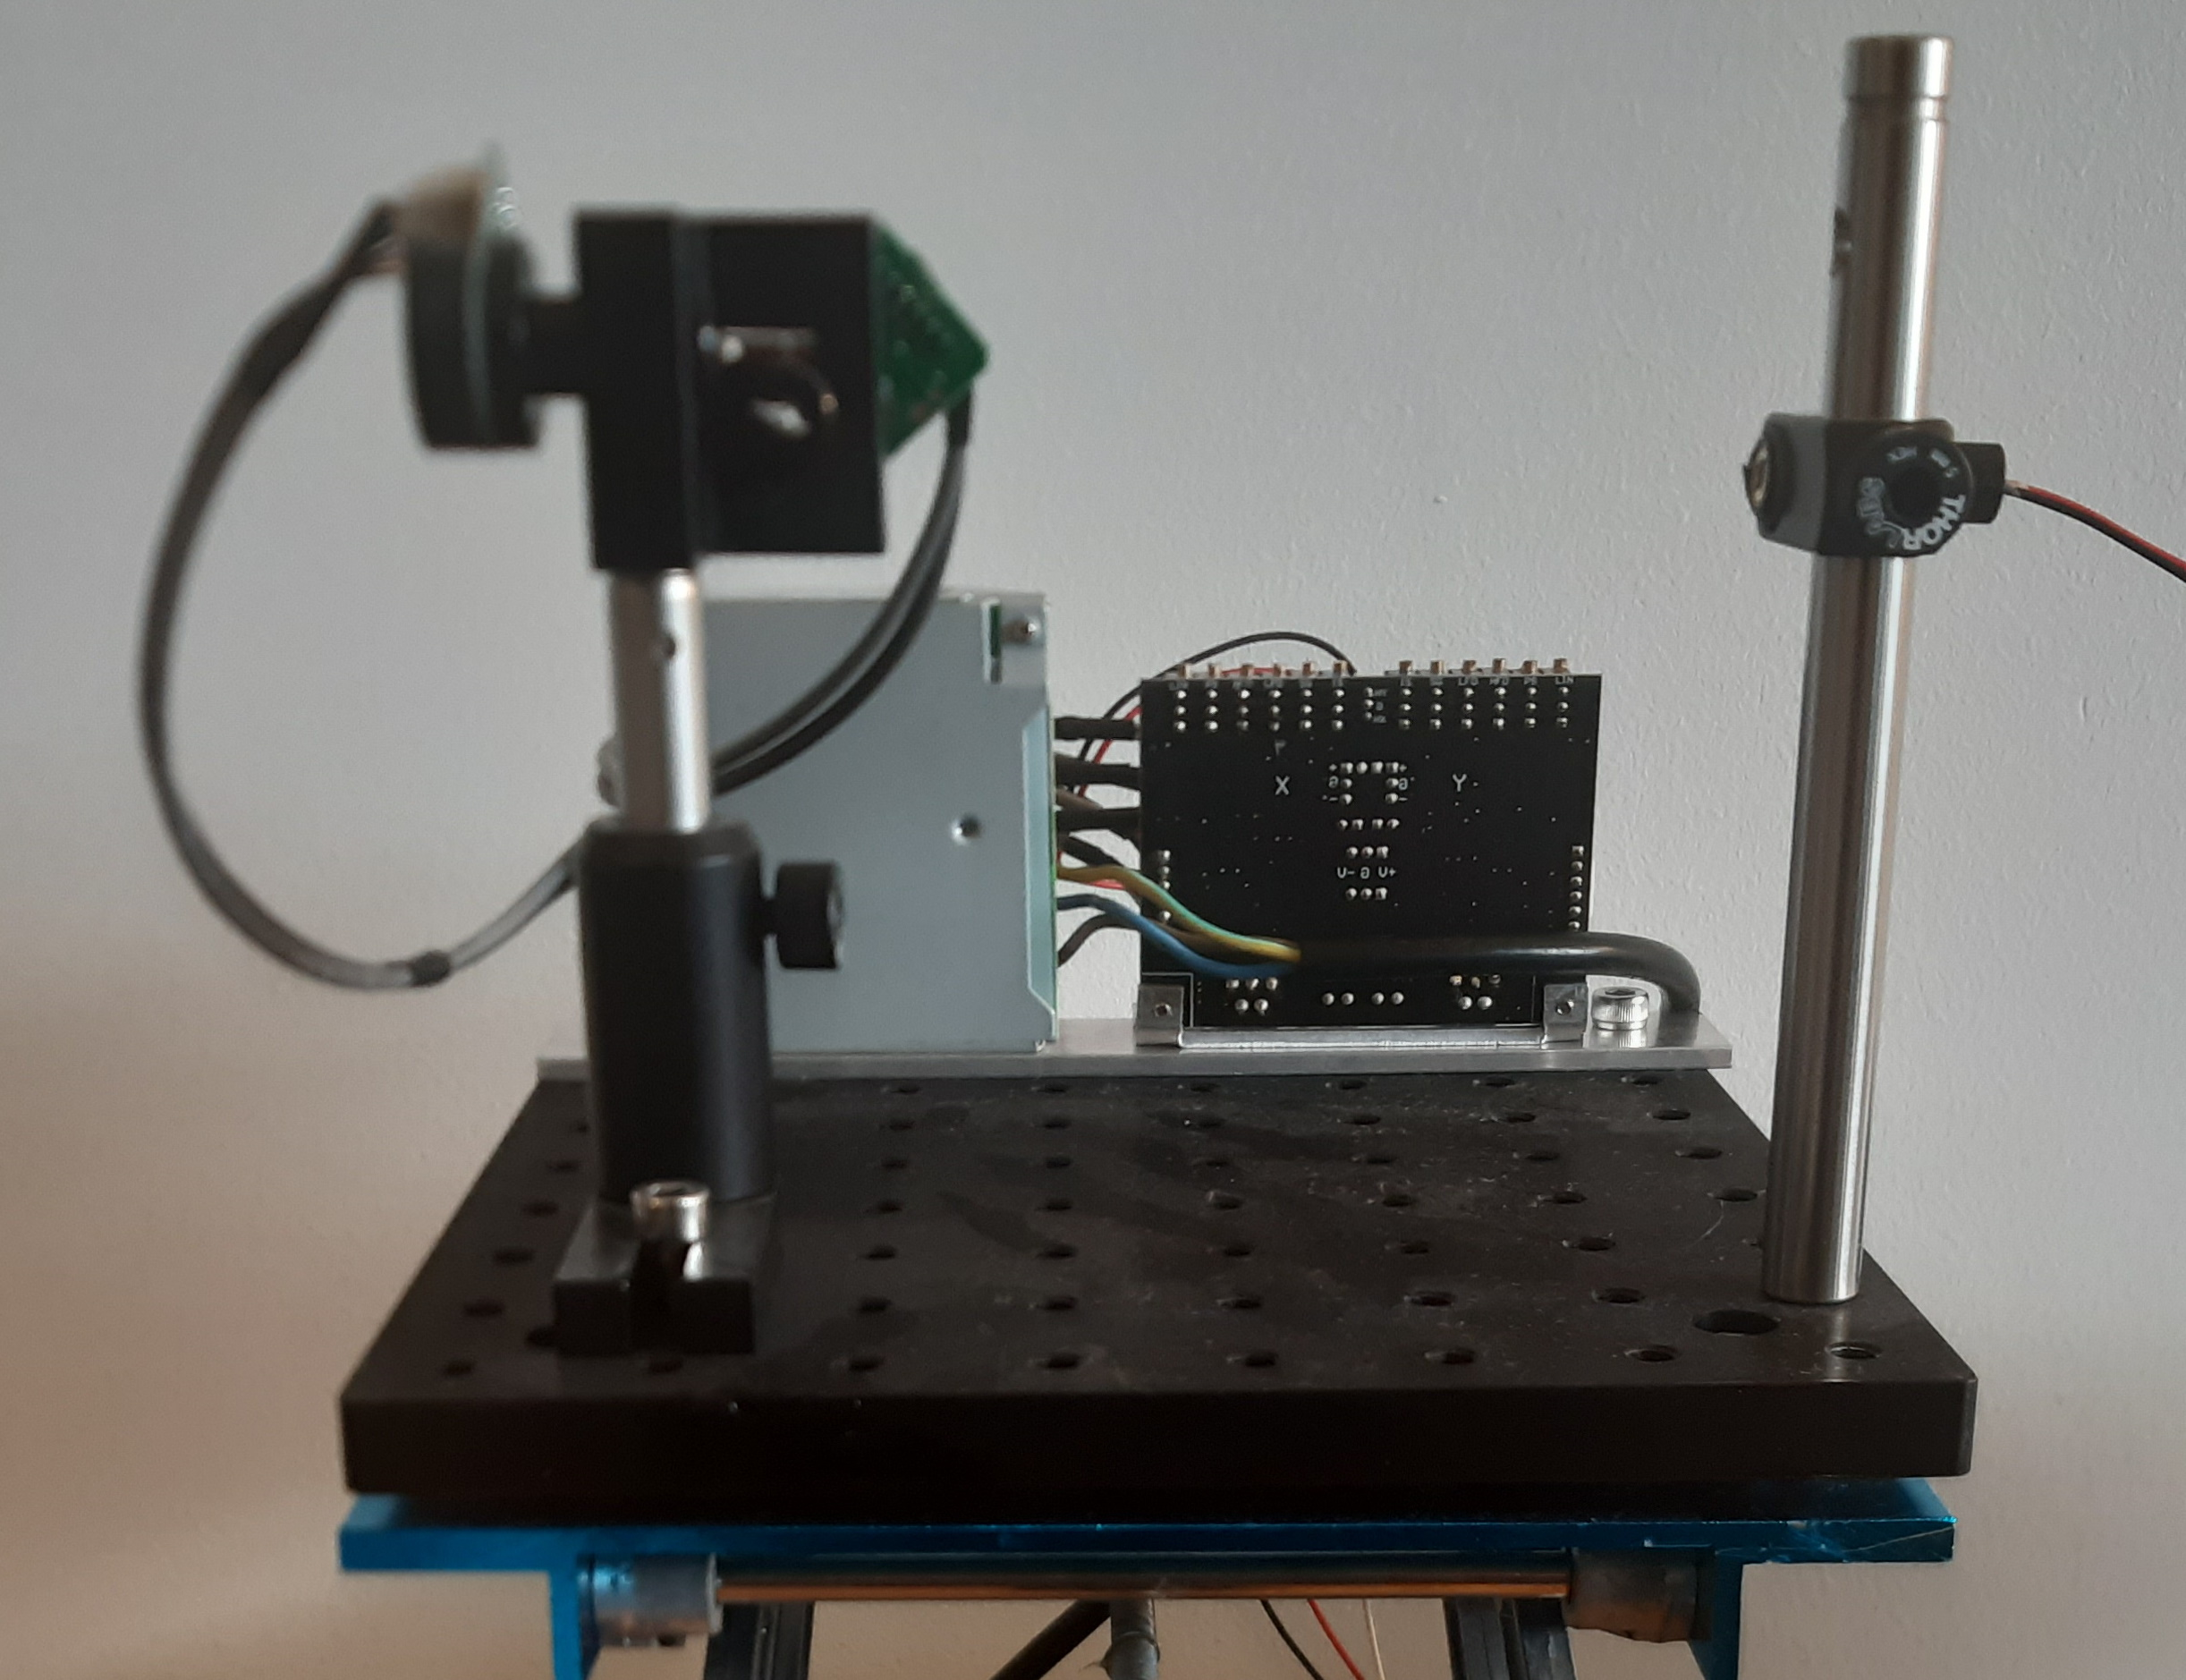
\includegraphics[width=\bildwidth]{pics/DutFront01.jpg}	\caption{DutFront01}	\label{DutFront01}	\end{figure}
% \begin{figure}[h!]	\centering	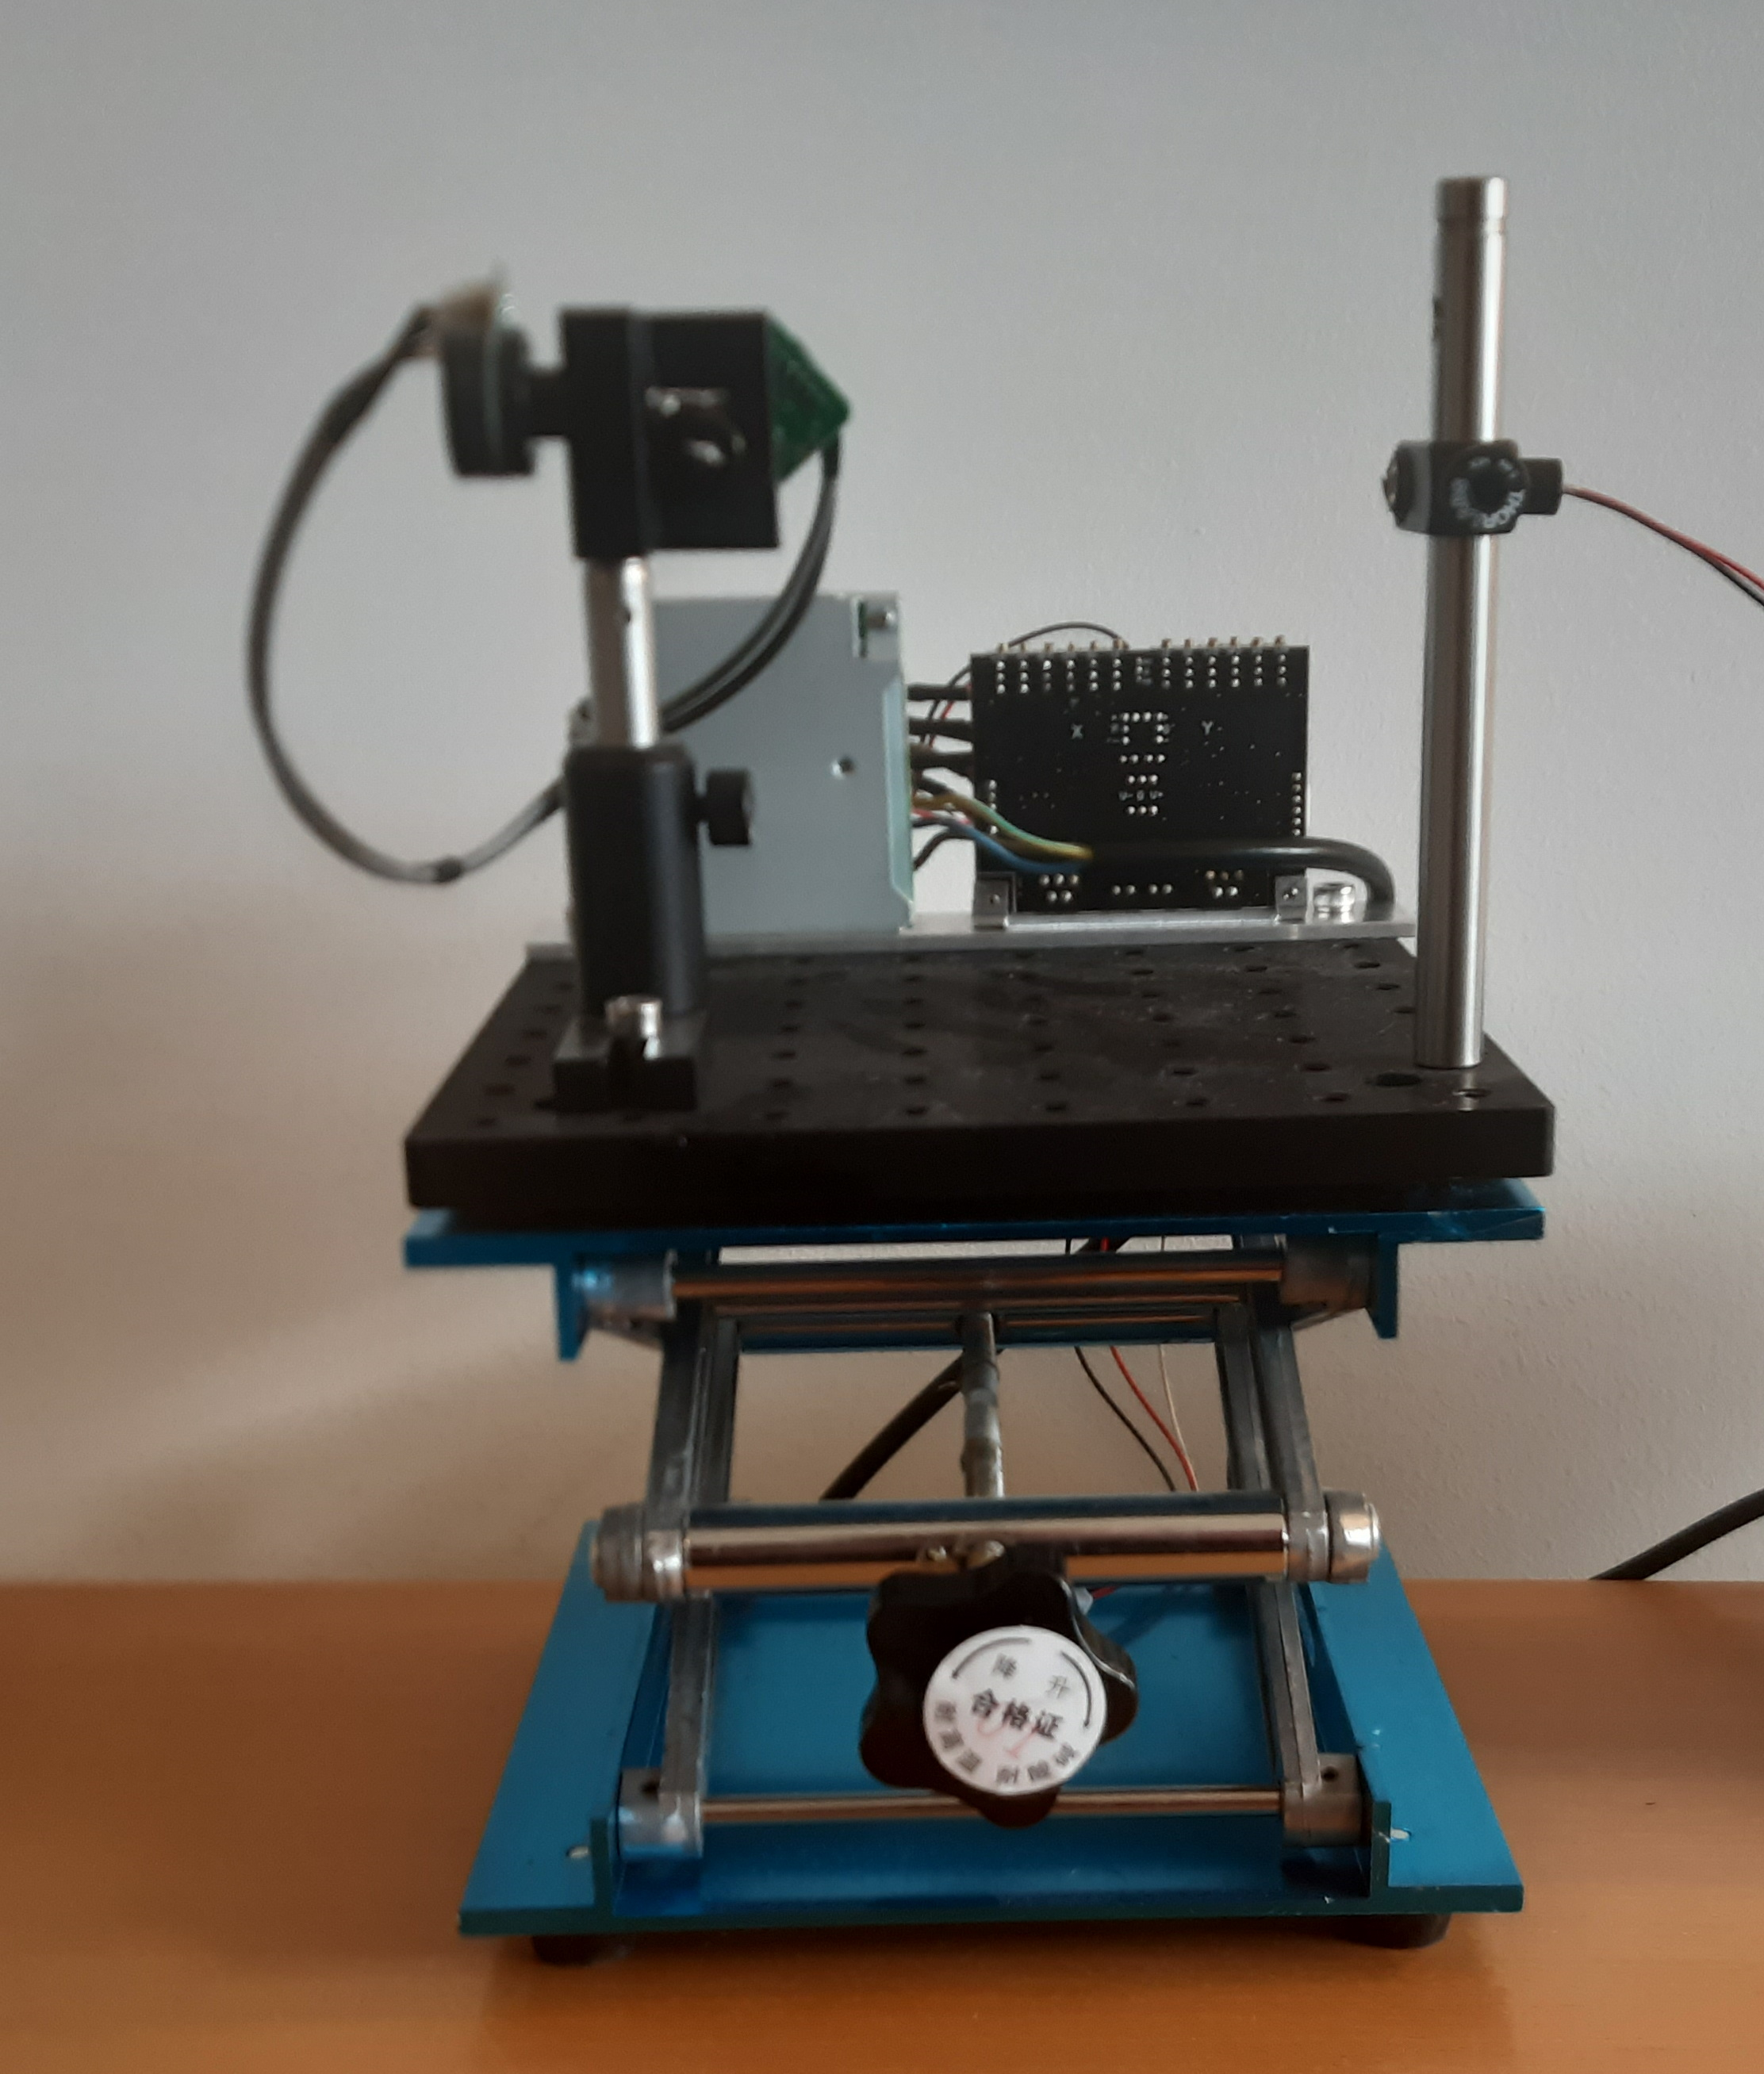
\includegraphics[width=\bildwidth]{pics/DutFront02.jpg}	\caption{DutFront02}	\label{DutFront02}	\end{figure}
% \begin{figure}[h!]	\centering	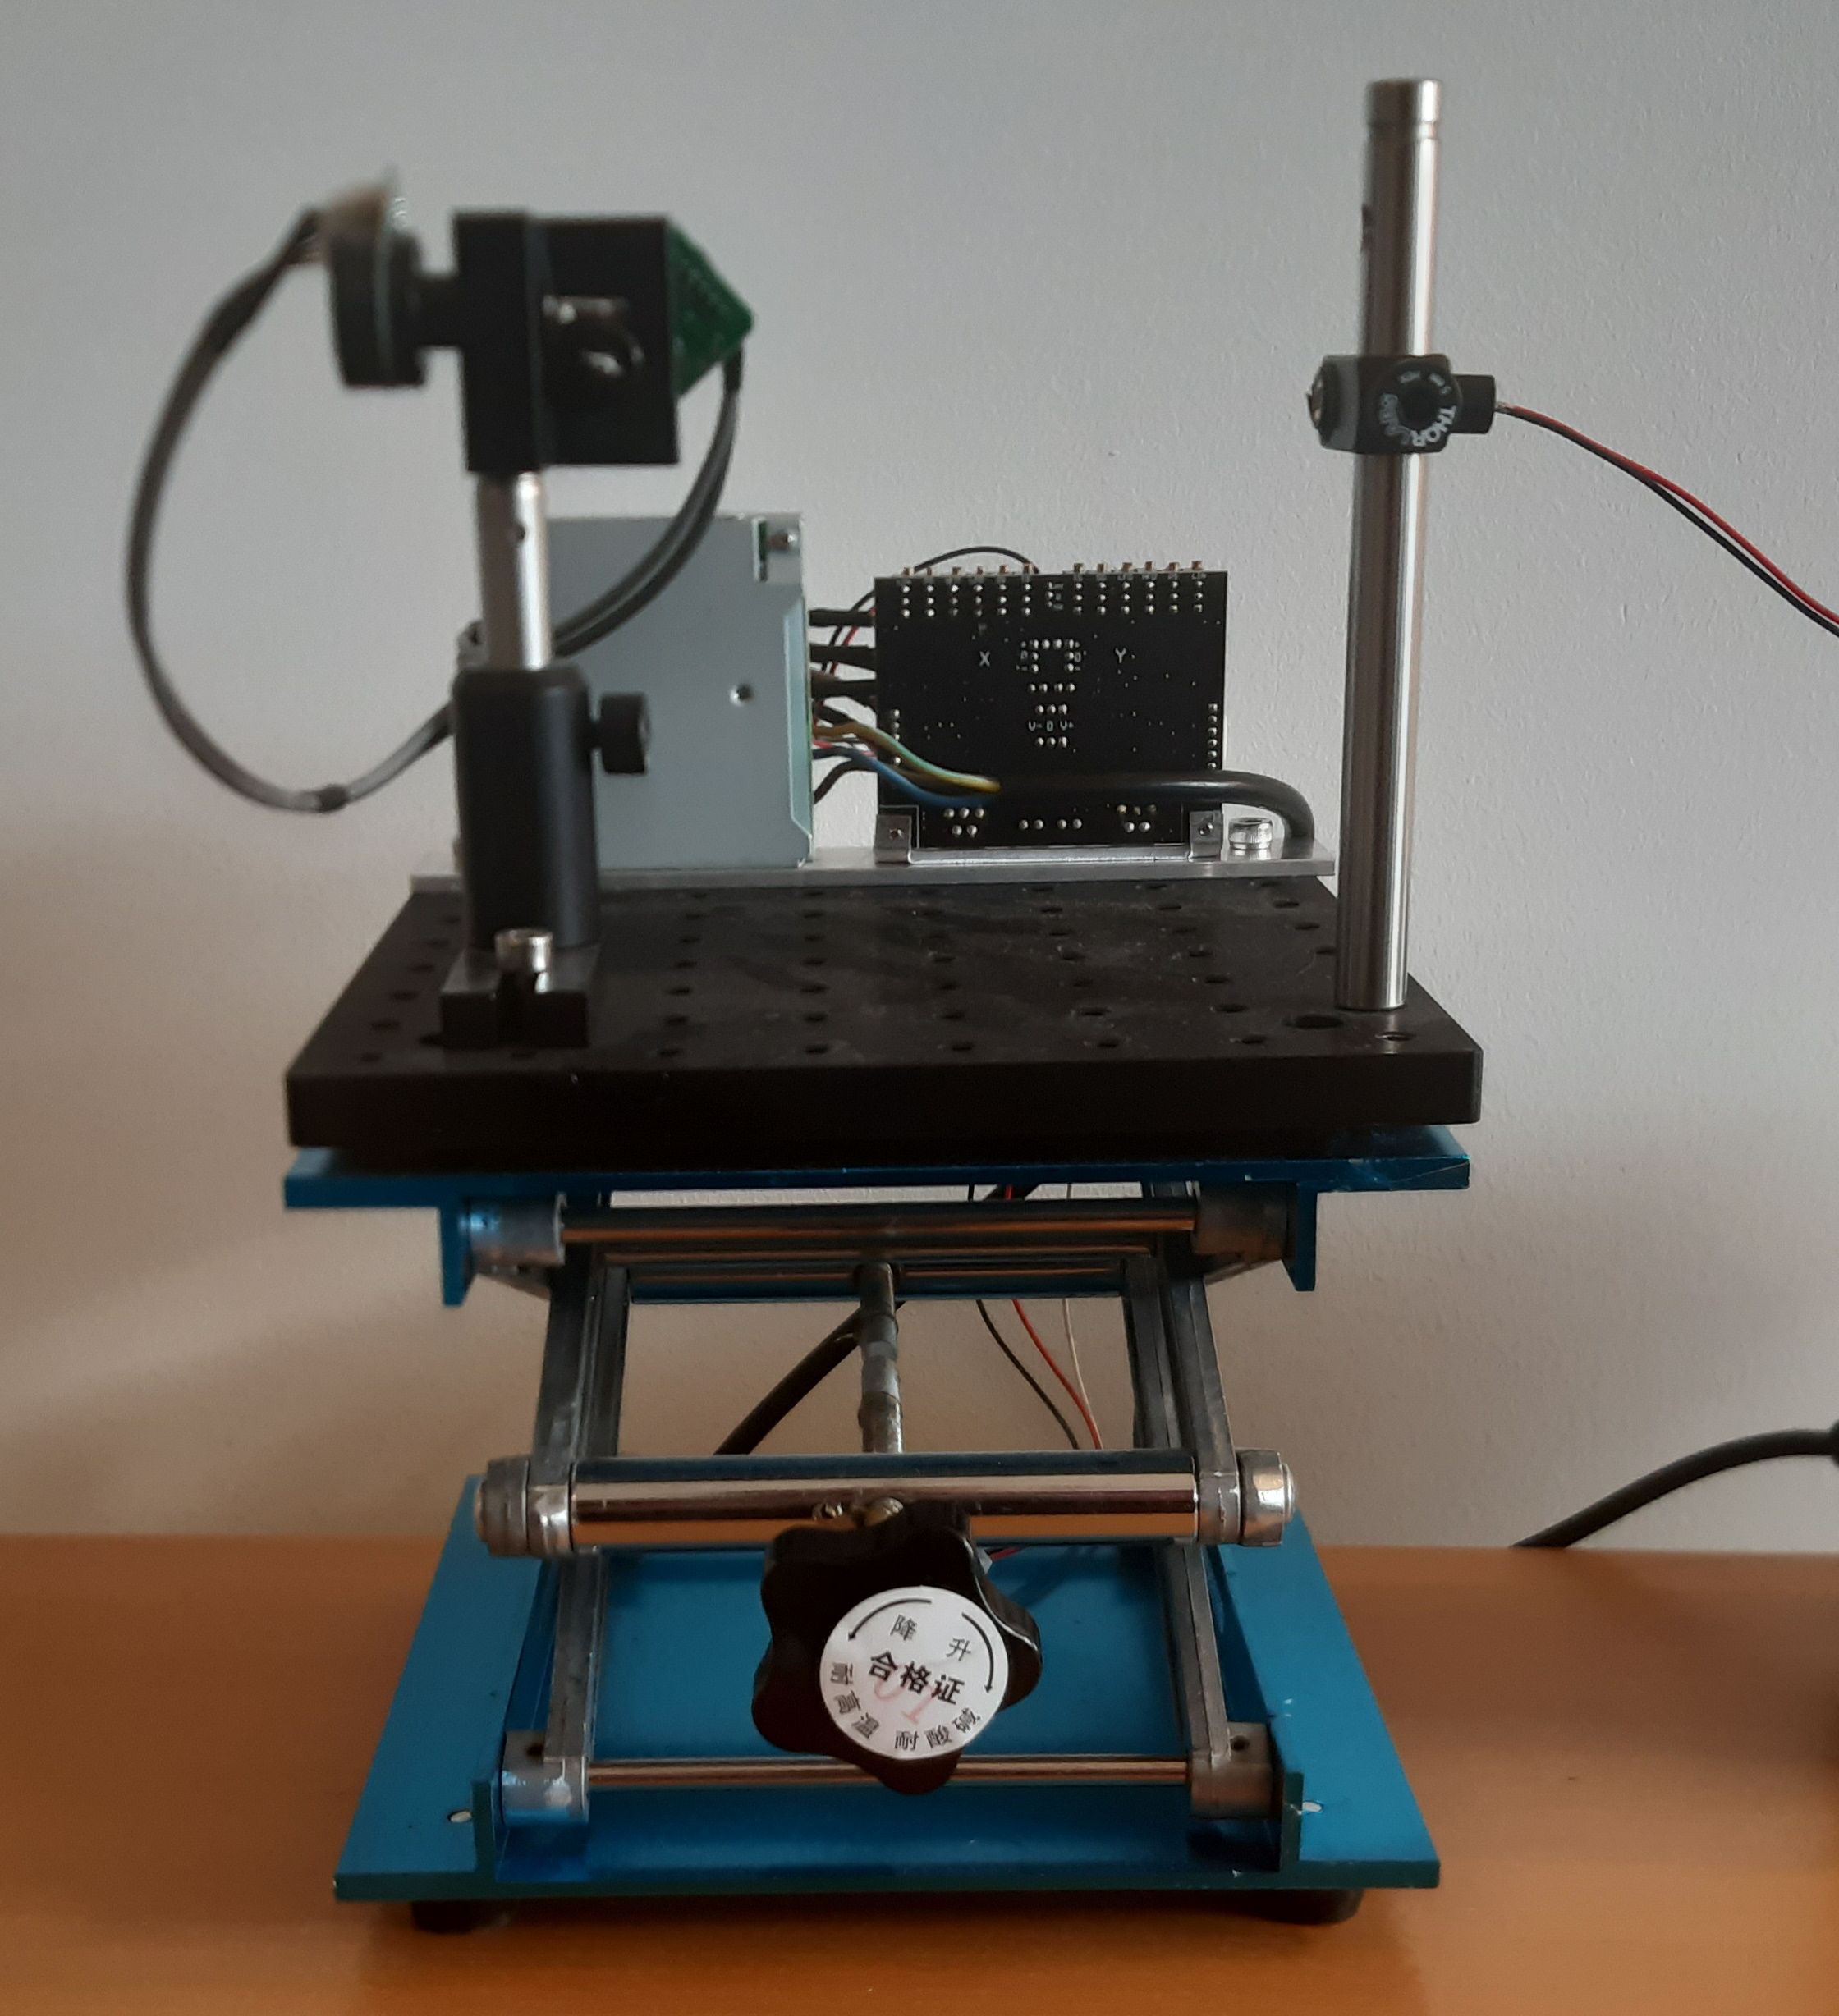
\includegraphics[width=\bildwidth]{pics/DutFront03.jpg}	\caption{DutFront03}	\label{DutFront03}	\end{figure}
% \begin{figure}[h!]	\centering	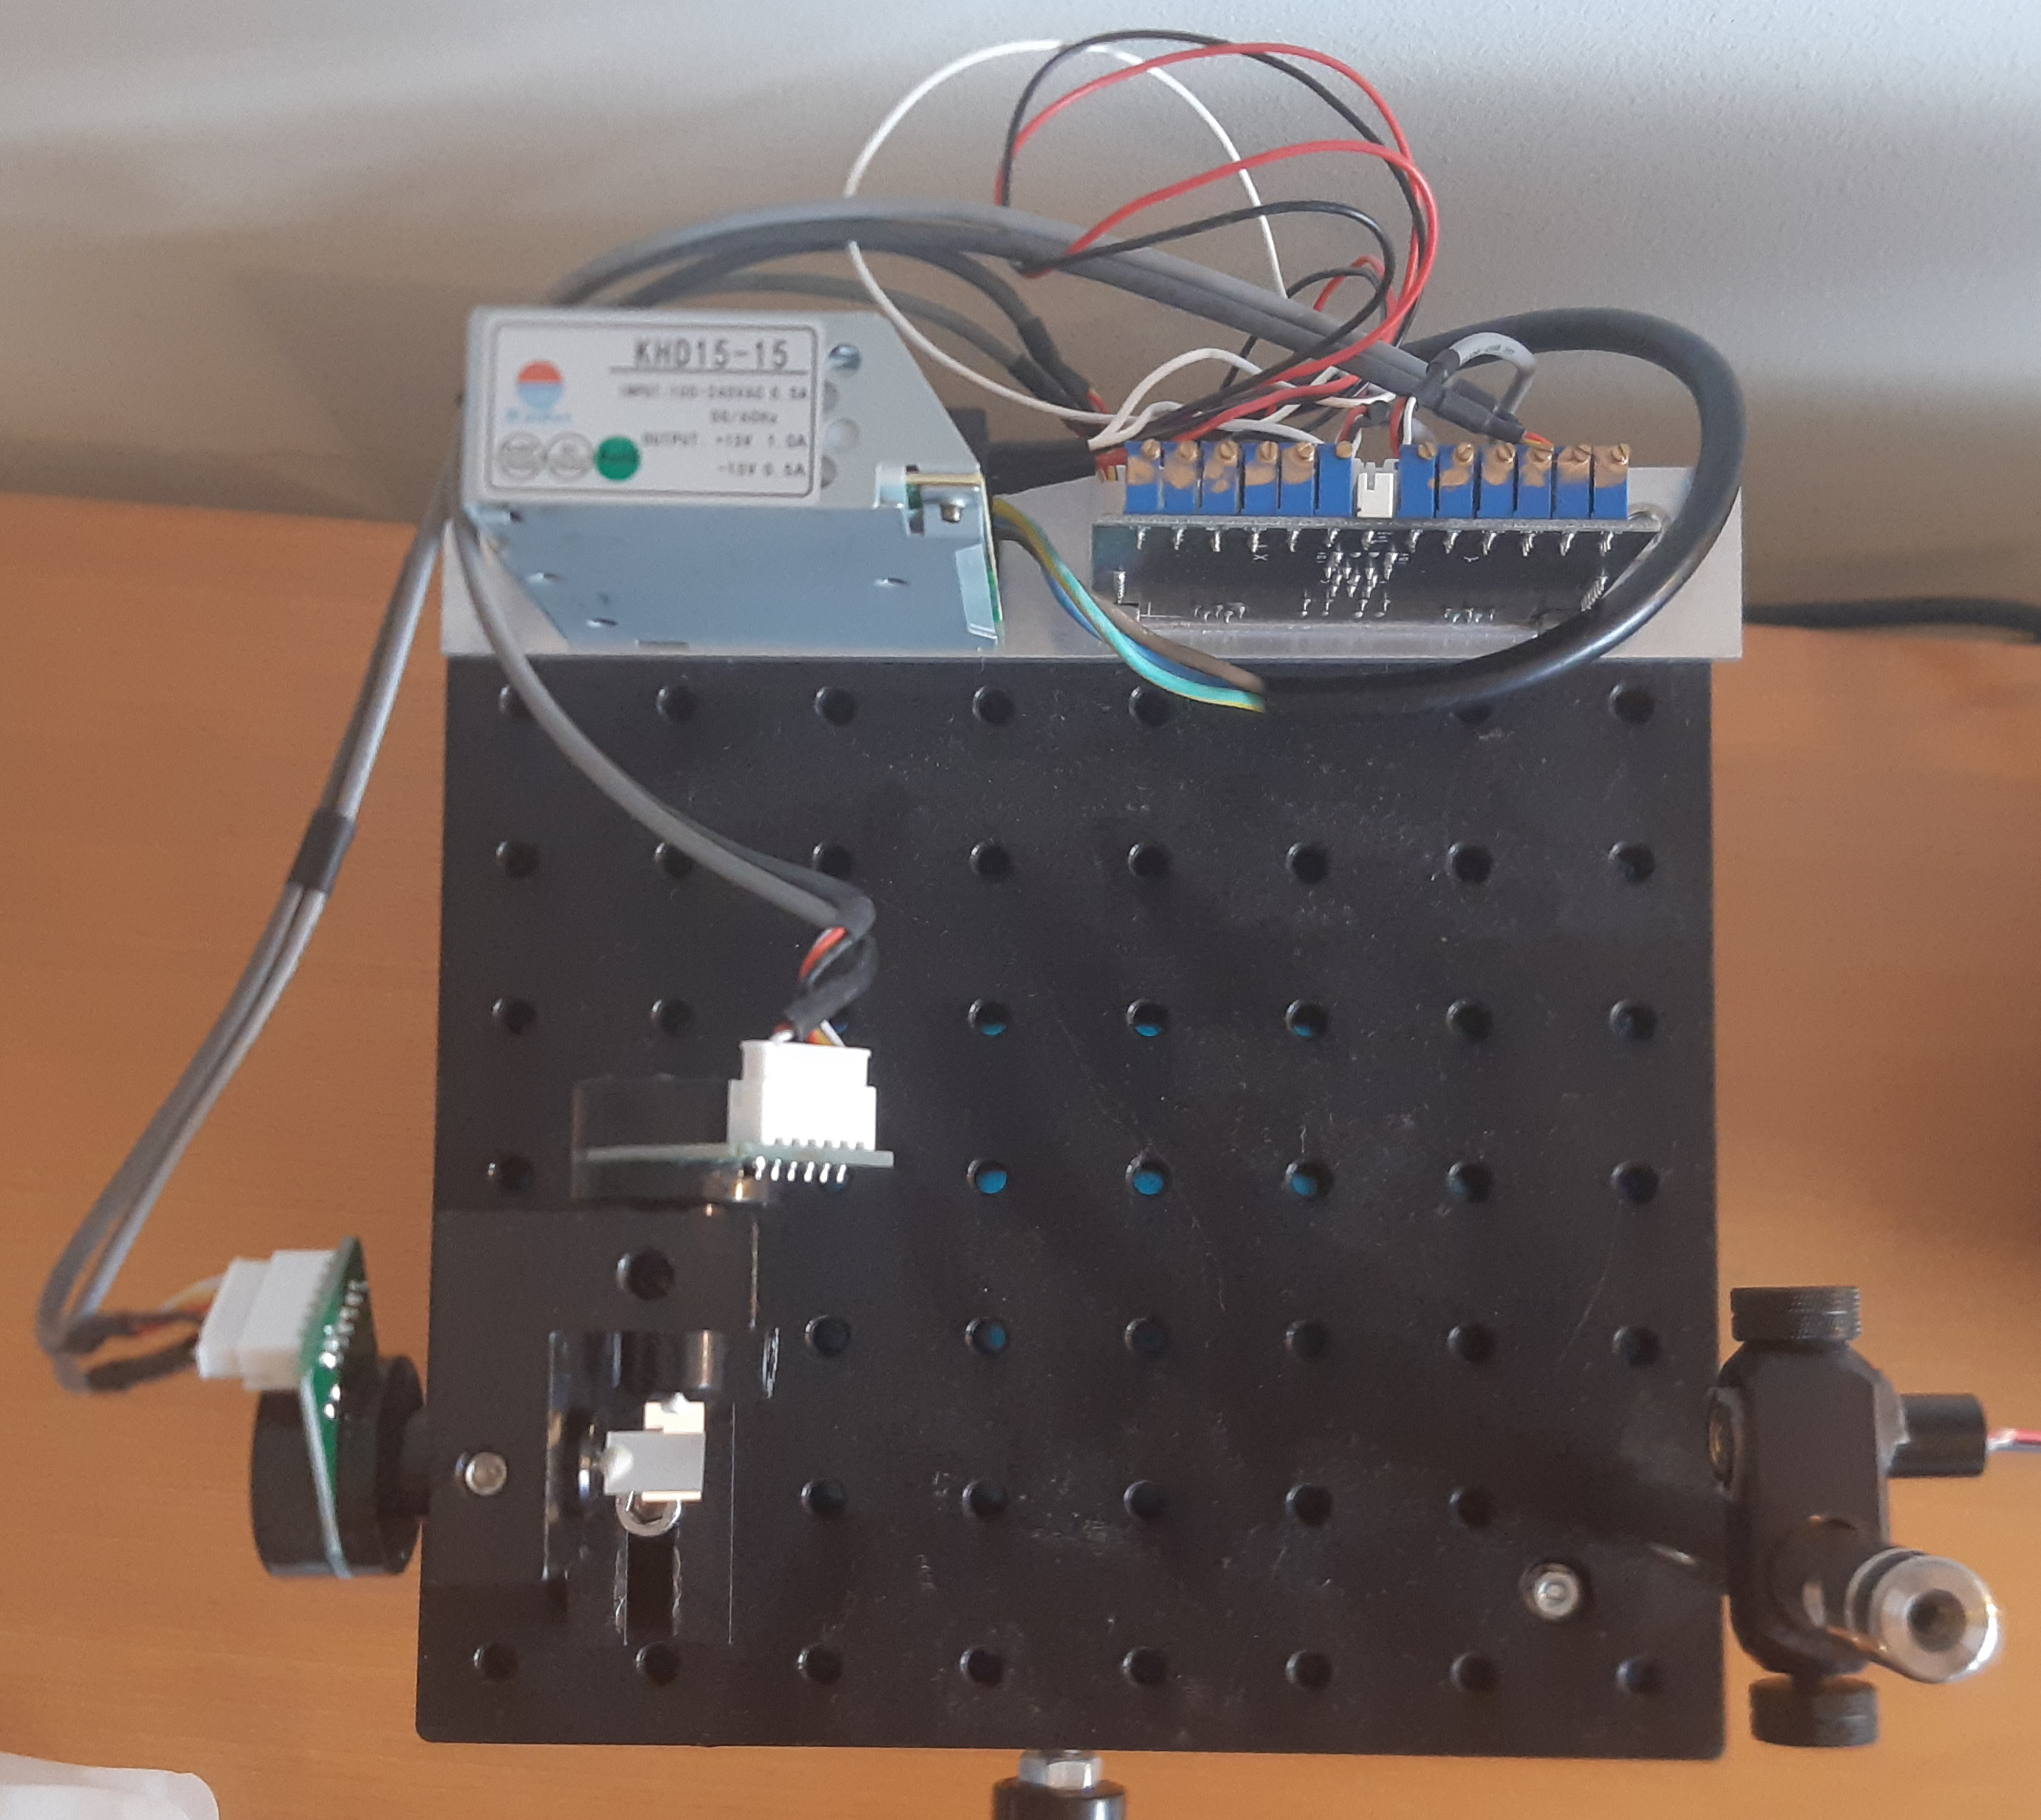
\includegraphics[width=\bildwidth]{pics/DutTop01.jpg}	\caption{DutTop01}	\label{DutTop01}	\end{figure}
\begin{figure}[h!]	\centering	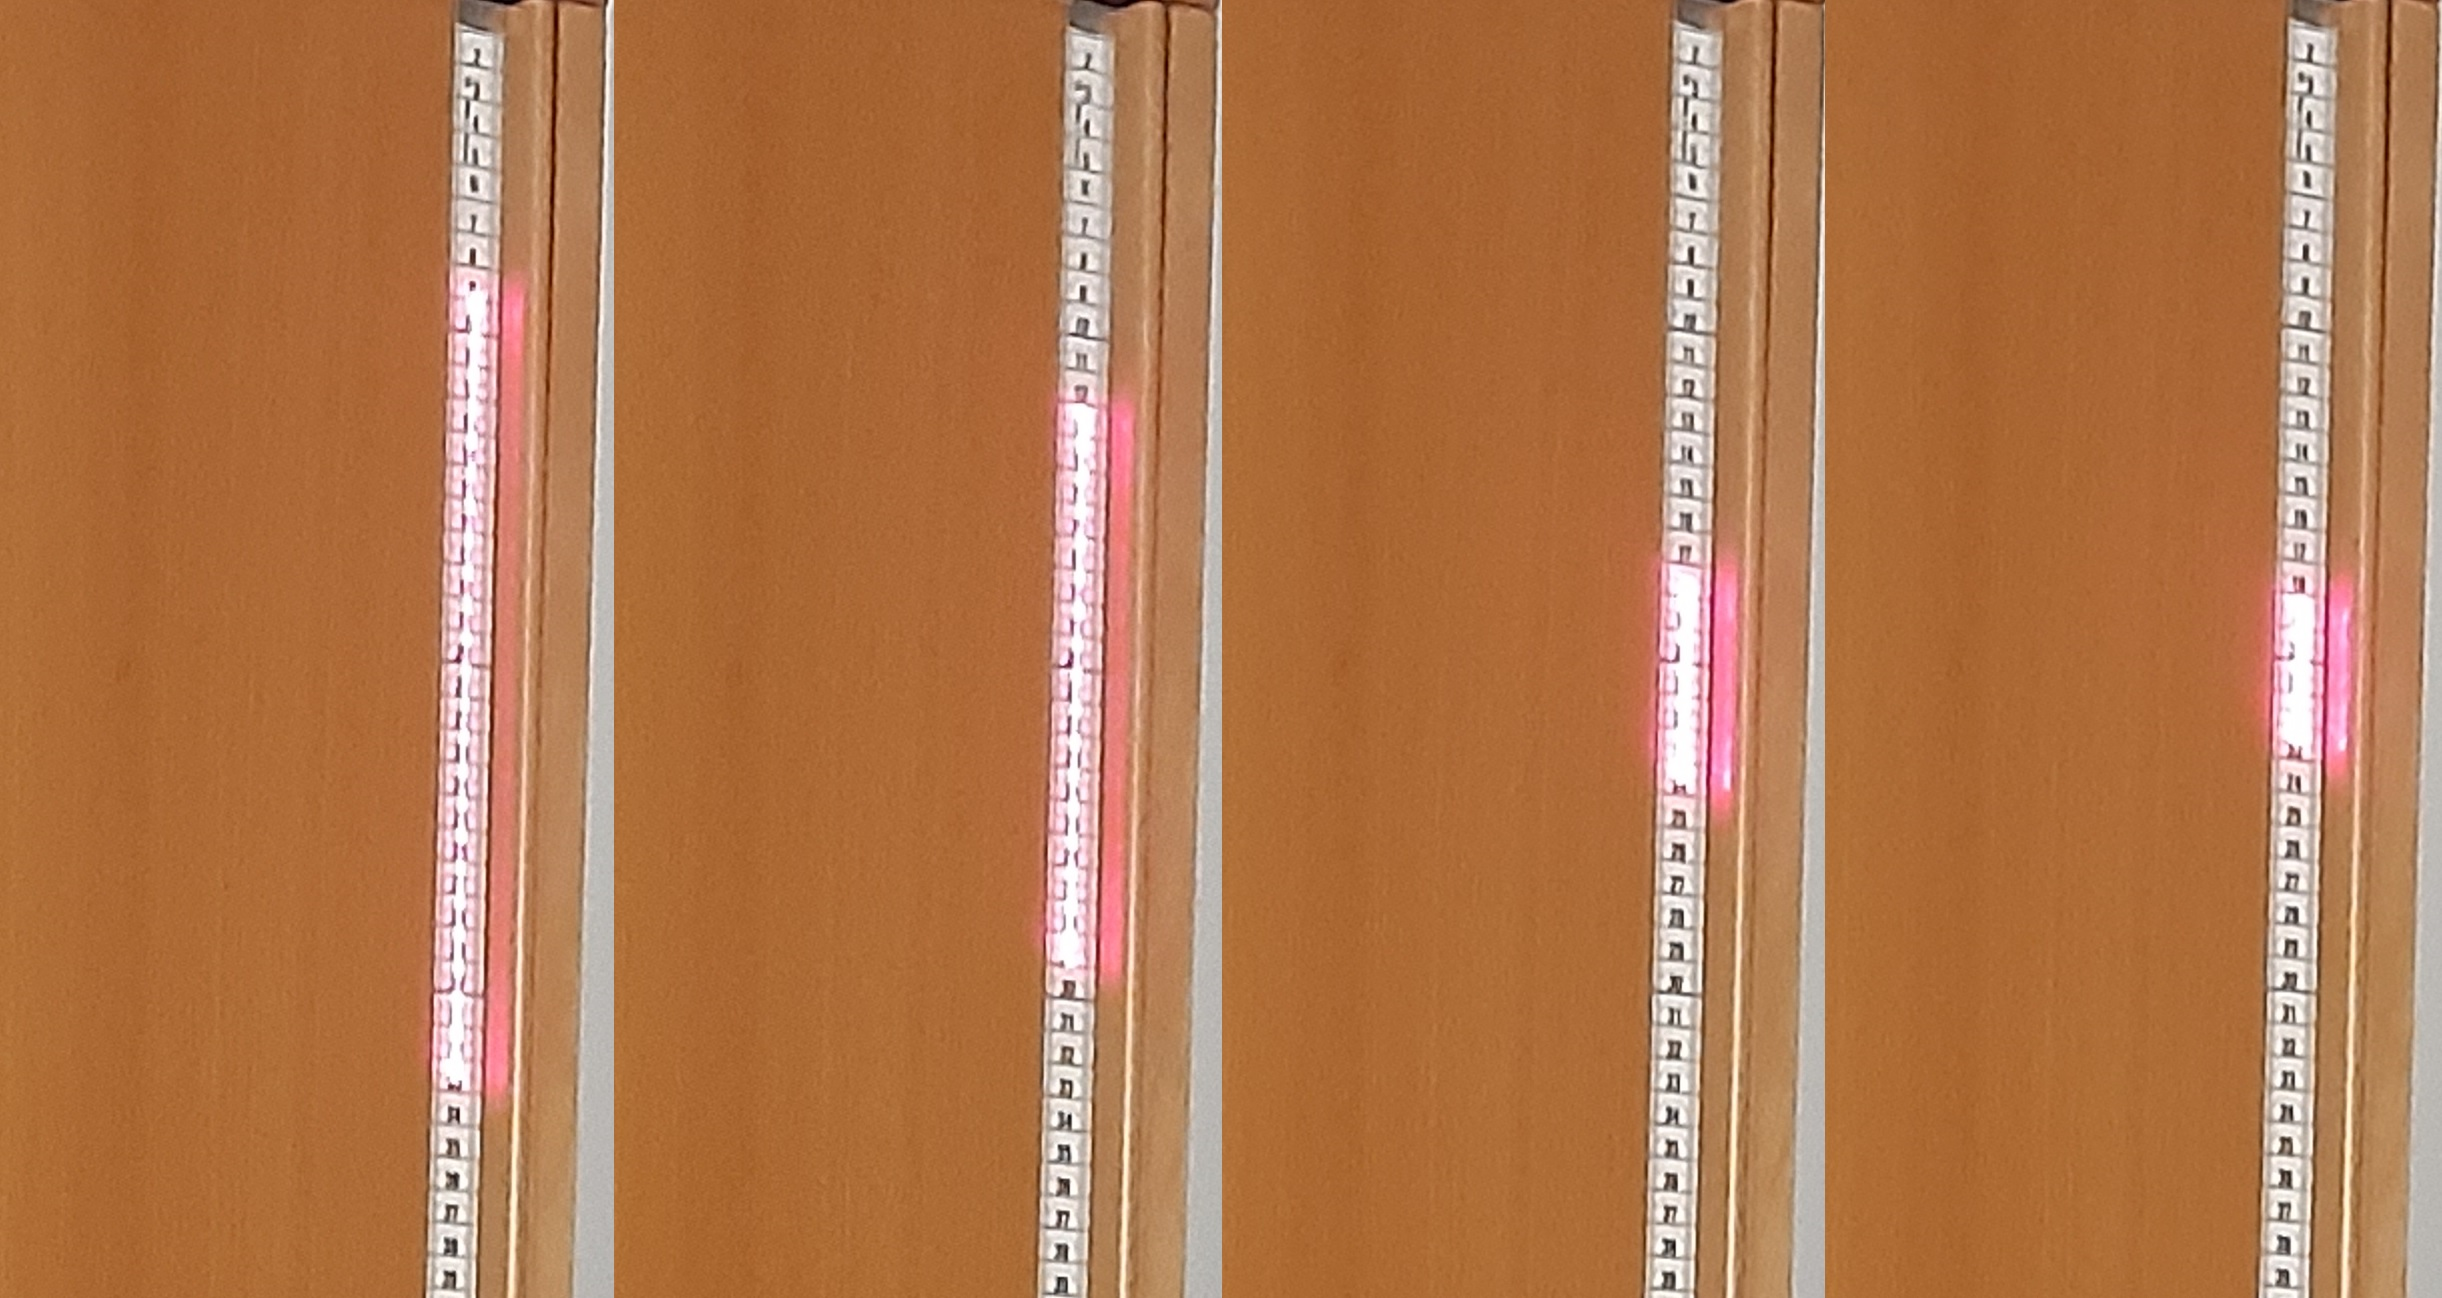
\includegraphics[width=\bildwidth]{pics/ImageMeasure01.jpg}	\caption{Abbilder von vier Messungen}	\label{ImageMeasure01}	\end{figure}
\bild{h!}{DetektorsForPhase}{Detektor zur Phasenmessung}{DetektorsForPhase}
% \begin{figure}[h!]	\centering	
\includegraphics[width=\bildwidth]{pics/ImageXY01.jpg}	\caption{ImageXY01}	\label{ImageXY01}	\end{figure}
% \begin{figure}[h!]	\centering	\includegraphics[width=\bildwidth]{pics/.jpg}	\caption{}	\label{fig_sim}	\end{figure}

% \subsection{Messungen}
	% \begin{table}[h!]
	% \begin{center}
	% \begin{tabular}{l|l}
	% \input{Mess1.csv}
	% \end{tabular}
	% \caption{Messungcsv}
	% \label{Messungcsv}
	% \end{center}
	% \end{table}

\section{Ergebnisse}
\bild{h!}{Mess1log.eps}{Bode-Diagramm des \galvo }{Mess1log}
Die Ergebnisse der Messung sind in Abb.~\ref{Mess1log} dargestellt: Es existiert ein linearer Bereich unterhalb von 1kHz, bei dem die Auslenkung sehr exakt dem Steuersignal folgt. Oberhalb davon nimmt die Auslenkung mit steigender Frequenz ab und erreicht beim orangen Marker die -3dB-Grenzfrequenz mit 1.3kHz. Zwischen dem gruenen und roten Marker verdoppelt sich die Frequenz, was einer Oktave entspricht. Die Amplitude der Auslenkung faellt dabei um 6.43dB. Diese naeherungsweise 6dB/Oktave entsprechen 40dB/Dekade und somit einem System zweiter Ordnung der Form\cite{Staudecker}
	\begin{align*}
	% G(s) & = \frac{V}{(T_N s)^2 + 2 \xi T_N s +1} & \textrm{wird mit} \\
	% |s| & = |\alpha + j\omega| \overset{\alpha = 0} = \omega & \textrm{und} \\
	% T_N & = \frac{1}{\omega_0}  & 	\textrm{zu} \\
	G(\omega) & = \frac{V}{(\frac{\omega}{\omega_0} )^2 + 2 \xi \frac{\omega}{\omega_0}  +1} & \textrm{mit} \\
	% d &= 3190 mm \\
	\xi & = 1 \\
	\omega_0 &= 2\pi f_g \\
	f_{g}	& = 1300 Hz \\
	V &= 116.4 \frac{mm}{V} \\ % =  291mm/2.5V
	% dmax = 291mm
	% Vpp = 2.5V
	% f_{g,1Vpp} & = 1000 Hz \\
	\end{align*}
Die Daempfung $\xi$ mit '1' laesst sich aus dem Kurvenverlauf abschaetzen, da dieser keine Resonanzspitze an der Grenzfrequenz aufweist. Die Verstaerkung 'V' setzt die maximale Auslenkung mit der Amplitude der Steuerspannung ins Verhaeltnis. Auf eine Rueckrechnung von der Auslenkung auf den Drehwinkel des \galvo s wurde verzichtet. Fuer die Applikation ist die erreichbare Auslenkung in mm von Bedeutung, der Winkel stellt somit keine relevante Information dar. Beide vorhandenen  Galvanometer-Spiegel des Testobjektes wurden unter gleichen Bedingungen vermessen und zeigten nahezu identes Verhalten bezueglich ihrer Dynamik. Das Phasendiagramm ergibt sich mit der Formel \textrm{$\phi = 360^\circ f  \Delta t$} aus den gemessenen $\Delta t$. Diese wiederum stellen die Verzoegerung zwischen dem Nulldurchgang des Steuersignals, sowie der steigenden Flanke eines Opto-Detektors dar, der an der optischen Null-Position platziert ist. Der resultierende Verlauf entspricht einigermassen dem erwarteten Phasengang eines Systems 2ter Ordnung. Allerdings weist er schon bei tiefen Frequenzen eine Abweichung von der 0grad-Achse ab, was eine Totzeit des verwendeten Detektors vermuten laesst.
\section{Konklusion}
Das gewonnene Modell wird in einer Masterarbeit zur Adaptierung von Steuersignalen herangezogen. Das zugrundeliegende Konzept dazu nennt sich 'flachheitsbasierte Steuerung'. Hierbei wird das Steuersignal, unter Einbeziehung der Modell-Eigenschaften, so berechnet, dass der Ausgang einer Sollkurve folgt. Abgesehen von diesem direkten Nutzen der Messungen, verbessert sich auch das intuitive Verstaendnis der analysierten Komponenten und nuetzt damit bei der Applikation und Abschaetzung der Applizierbarkeit in OCT-Systeme. \\
Weitere Messungen mit unterschiedlichen Steuerspannungen und an mehreren Frequenzen, 	speziell im Bereich der Grenzfrequenz, sollen das bestehende Modell noch verfeinern. Auch soll die vermutete Totzeit des Opto-Detektors untersucht werden, damit praezisere Phasen-Messungen moeglich sind.

% \hfill rechtsbuendiger Text
\section*{Danksagung}
% \begin{itemize}
Martin Staudecker, Guenther Hannesschlaeger, Rankl Christian, Josef Langer und Silke Dorner, fuer die Assistenz bei Messungen.
% \end{itemize}
\label{cha:galvoChar}

% \chapter{Closing Remarks}
\label{cha:Closing}

%%%-----------------------------------------------------------------------------
\appendix                                                             % Appendix 
%%%-----------------------------------------------------------------------------

\chapter{Technical Details}
\label{app:TechnicalDetails}



 % Technical supplements
\chapter{Supplementary Materials}
\label{app:materials}


List of supplementary data submitted to the degree-granting institution for archival storage
(in ZIP format).

% Use this as an example only, adapt the structure to your requirements!

\section{PDF Files}
\begin{FileList}{/}
\fitem{thesis.pdf} Master/Bachelor thesis (complete document)
\end{FileList}

\section{Media Files}
\begin{FileList}{/media}
\fitem{*.ai, *.pdf} Adobe Illustrator files
\fitem{*.jpg, *.png} raster images
\fitem{*.mp3} audio files
\fitem{*.mp4} video files
\end{FileList}


% \section{Online Sources (PDF Captures)}
% \begin{FileList}{/online-sources}
% \fitem{Reliquienschrein-Wikipedia.pdf} \parencite{WikiReliquienschrein2020}
% \end{FileList}




 % Contents of the CD-ROM/DVD
\chapter{Questionnaire}
\label{app:Questionnaire}





 % Chronological list of changes
\chapter{\latex Source Code}
\label{app:SourceCode}

 % Source text of this document

%%%-----------------------------------------------------------------------------
\backmatter                           % Back part (bibliography, glossary, etc.)
%%%-----------------------------------------------------------------------------

\MakeBibliography % References

%%%-----------------------------------------------------------------------------
% Special page for checking print size
%%%-----------------------------------------------------------------------------

% \chapter*{Check Final Print Size}

\begin{center}
{\Large --- Check final print size! ---}

\bigskip

\calibrationbox{100}{50} % width/height of box in mm

\bigskip

{\Large --- Remove this page after printing! ---}

\end{center}



%%%-----------------------------------------------------------------------------
\end{document}
%%%-----------------------------------------------------------------------------
